\documentclass[11pt,a4paper]{article}

% Pacotes essenciais
\usepackage[utf8]{inputenc}
\usepackage[T1]{fontenc}
\usepackage{lmodern}
\usepackage[portuguese]{babel}
\usepackage{graphicx}
\usepackage{amsmath}
\usepackage{amsfonts}
\usepackage{amssymb}
\usepackage{float}
\usepackage{caption}
\usepackage{subcaption}
\usepackage{xcolor}
\usepackage{colortbl}
\usepackage{fancyhdr}
\usepackage{geometry}
\usepackage{titlesec}

\usepackage[hidelinks]{hyperref}
\usepackage[alf]{abntex2cite}
\usepackage{booktabs}
\usepackage{array}
\usepackage{pdflscape}

\usepackage{enumitem}
\usepackage{tikz}


% Definição das cores
\definecolor{headercolor}{HTML}{b11116}
\definecolor{secondarycolor}{HTML}{3a5461}
\definecolor{primaryA}{HTML}{AED5FF}
\definecolor{primaryB}{HTML}{FFC2C2}

% Configuração da página
\geometry{
    a4paper,
    top=2.8cm,
    bottom=2.5cm,
    left=2.5cm,
    right=2.5cm,
    headheight=1.2cm,
    headsep=0.5cm
}

% Configuração do cabeçalho
\pagestyle{fancy}
\fancyhf{}
\renewcommand{\headrulewidth}{0pt}
\renewcommand{\footrulewidth}{0.5pt}

\fancyhead[L]{%
    \begin{tikzpicture}[remember picture, overlay]
        \fill[headercolor] (current page.north west) rectangle ([yshift=-1.2cm]current page.north east);
        \node[anchor=west, inner sep=0pt] at ([xshift=1cm, yshift=-0.6cm]current page.north west) 
            {
\includegraphics[height=0.8cm]{imgs/base/fatec-rgt.png}};
        \node[anchor=east, inner sep=0pt] at ([xshift=-1cm, yshift=-0.6cm]current page.north east) 
            {
\includegraphics[height=0.9cm]{imgs/base/cps-logo.png}};
        \node[anchor=east, inner sep=0pt] at ([xshift=-2.8cm, yshift=-0.6cm]current page.north east) 
            {
\includegraphics[height=1.05cm]{imgs/base/governo-sp-secretaria-logo.png}};
    \end{tikzpicture}
}

\fancyfoot[L]{\footnotesize\textcolor{secondarycolor}{Faculdade de Tecnologia do Estado de São Paulo\\ fatecregistro.cps.sp.gov.br}}
\fancyfoot[R]{\thepage}

% Configuração dos títulos das seções
\titleformat{\section}
    {\normalfont\large\bfseries\color{secondarycolor}}
    {\thesection}{1em}{}

\titleformat{\subsection}
    {\normalfont\normalsize\bfseries\color{secondarycolor}}
    {\thesubsection}{1em}{}

\begin{document}

% ===== CAPA =====
\begin{titlepage}
    \centering
    
    \begin{tikzpicture}[remember picture, overlay]
        \fill[headercolor] (current page.north west) rectangle ([yshift=-1.2cm]current page.north east);
        \node[anchor=west, inner sep=0pt] at ([xshift=1cm, yshift=-0.6cm]current page.north west) 
            {
\includegraphics[height=0.8cm]{imgs/base/fatec-rgt.png}};
        \node[anchor=east, inner sep=0pt] at ([xshift=-1cm, yshift=-0.6cm]current page.north east) 
            {
\includegraphics[height=0.9cm]{imgs/base/cps-logo.png}};
        \node[anchor=east, inner sep=0pt] at ([xshift=-2.8cm, yshift=-0.6cm]current page.north east) 
            {
\includegraphics[height=1.05cm]{imgs/base/governo-sp-secretaria-logo.png}};
    \end{tikzpicture}
    
    \vspace*{3.5cm}
    
    {\normalsize FACULDADE DE TECNOLOGIA DO ESTADO DE SÃO PAULO\par}
    \vspace{0.5cm}
    
    {\normalsize DESENVOLVIMENTO DE SOFTWARE MULTIPLATAFORMA\par}
    
    \vspace{4cm}
    
    {\normalsize ARTEFATOS DO PROJETO DE SOFTWARE\par}
    
    \vspace{0.3cm}
    
    {\normalsize Criação de Camarão em Cativeiro com Monitoramento IoT para Gastronomia\par}
    
    \vspace{3cm}
    
    {\normalsize
    Davi Mathais de Almeida\\
    Leandro Augusto De Souza Muniz\\
    Tiago de Lara Rodrigues
    }
    
    \vfill
    
    {\small Registro -- SP\\
    2026}
    
\end{titlepage}

\pagestyle{fancy}

% ===== SUMÁRIO =====
\tableofcontents
\newpage

\subsection*{Lista de Artefatos e suas Finalidades}

\begin{itemize}
    \item \textbf{CANVAS:} Modelo de negócio e estratégia
    \item \textbf{SWOT:} Análise estratégica de forças, fraquezas, oportunidades e ameaças
    \item \textbf{UX/UI:} Design de interface e experiência do usuário
    \item \textbf{Website:} Estrutura e especificações técnicas web
    \item \textbf{Diagramas UML:} Modelagem visual do sistema
    \item \textbf{DevOps:} Infraestrutura, automação e práticas de entrega contínua
\end{itemize}

\vspace{0.5cm}
\noindent\rule{\textwidth}{0.5pt}

\newpage

% ===== CANVAS =====
\section{CANVAS: Modelo de Negócio e Estratégia}

O Business Model Canvas \cite{osterwalder2011} é uma ferramenta visual estratégica que permite descrever, analisar e projetar modelos de negócio de forma clara e objetiva. O canvas é dividido em nove blocos fundamentais que cobrem as principais áreas de um negócio.

\begin{table}[H]
\centering
\caption{Business Model Canvas -- Visão Geral}
\label{tab:canvas}
\small
\begin{tabular}{|p{2.5cm}|p{2.5cm}|p{2.8cm}|p{2.5cm}|p{2.8cm}|}
\hline
\textbf{Parcerias Principais} & \textbf{Atividades Chave} & \textbf{Proposta de Valor} & \textbf{Relacionamento} & \textbf{Segmentos} \\
\hline
Consultores da carcinicultura, produtores de camarão & Interpretação de dados sobre temperatura, pH e amônia, monitoramento comunicando com a plataforma & Automatização no cuidado dos cativeiros, redução de custos, aplicação juntamente com sistema IoT & Suporte técnico, treinamentos, chat direto com a empresa & Carcinicultura, aquicultura, sistema de monitoramento \\
\hline
 & \textbf{Recursos Principais} & & \textbf{Canais} & \\
\hline
 & Sensores de temperatura, pH e amônia, microcontrolador ESP32, dispensador automatizado de ração & & Comunicação via redes sociais, e-mail e telefone & \\
\hline
\multicolumn{2}{|p{5.5cm}|}{\textbf{Estrutura de Custos}} & \multicolumn{3}{p{7.5cm}|}{\textbf{Fontes de Receita}} \\
\hline
\multicolumn{2}{|p{5.5cm}|}{Desenvolvimento do sistema, equipamentos IoT, marketing} & \multicolumn{3}{p{7.5cm}|}{Plano de assinatura mensal e anual, treinamentos, instalação do sistema} \\
\hline
\end{tabular}
\end{table}

\subsection{Análise do Modelo de Negócio}

A análise do Canvas revela que a proposta de valor do projeto está diretamente alinhada ao segmento de mercado identificado: a automatização do cuidado dos cativeiros e a redução de custos operacionais atendem às necessidades dos produtores de camarão que atualmente dedicam em média cinco horas diárias ao manejo manual. As atividades-chave de interpretação de dados e monitoramento em tempo real são viabilizadas pelos recursos principais, notadamente o microcontrolador ESP32 e os sensores integrados, que constituem a base tecnológica do sistema. O modelo de receita baseado em assinaturas mensais e anuais garante previsibilidade financeira e permite a manutenção contínua do sistema, enquanto as parcerias com consultores da carcinicultura e produtores locais asseguram a validação técnica e a aderência da solução à realidade do setor. Os canais de comunicação via redes sociais, e-mail e telefone possibilitam tanto a aquisição de novos clientes quanto o suporte técnico aos produtores já cadastrados.

% ===== SWOT =====
\section{SWOT: Análise Estratégica}

A Análise SWOT (Strengths, Weaknesses, Opportunities, Threats) ou FOFA (Forças, Oportunidades, Fraquezas e Ameaças) \cite{chiavenato2020} é uma ferramenta fundamental para planejamento estratégico que permite identificar fatores internos e externos que impactam o projeto. Analisa forças, fraquezas, oportunidades e ameaças do projeto.

\begin{table}[H]
\centering
\caption{Análise SWOT do Projeto}
\label{tab:swot}
\begin{tabular}{|p{7.2cm}|p{7.2cm}|}
\hline
\multicolumn{2}{|c|}{\cellcolor{secondarycolor!20}\textbf{FATORES INTERNOS}} \\
\hline
\textbf{FORÇAS (Strengths)} & \textbf{FRAQUEZAS (Weaknesses)} \\
\hline
\begin{minipage}[t]{7cm}
\begin{itemize}
    \item Integração entre aplicação e sensores IoT em tempo real
    \item Automação de alimentação
    \item Sistema de alertas multicanal
    \item Interface intuitiva e responsiva
    \item Redução de custos operacionais
\end{itemize}
\end{minipage}
&
\begin{minipage}[t]{7cm}
\begin{itemize}
    \item Dependência de internet
    \item Necessidade de manutenção dos sensores
    \item Necessidade de treinamento dos usuários
    \item Custo inicial de implementação
\end{itemize}
\end{minipage}
\\
\hline
\multicolumn{2}{|c|}{\cellcolor{secondarycolor!20}\textbf{FATORES EXTERNOS}} \\
\hline
\textbf{OPORTUNIDADES (Opportunities)} & \textbf{AMEAÇAS (Threats)} \\
\hline
\begin{minipage}[t]{7cm}
\begin{itemize}
    \item Crescimento do mercado de aquicultura
    \item Parcerias com instituições de pesquisa
    \item Expansão para outros tipos de monitoramento ambiental
    \item Aumento da demanda por soluções sustentáveis
\end{itemize}
\end{minipage}
&
\begin{minipage}[t]{7cm}
\begin{itemize}
    \item Concorrência de soluções similares
    \item Resistência à adoção de novas tecnologias
    \item Cobertura \textit{Wi-Fi} limitada em propriedades rurais do Vale do Ribeira, exigindo soluções de conectividade alternativas
    \item Risco de falhas técnicas
\end{itemize}
\end{minipage}
\\
\hline
\end{tabular}
\end{table}

\subsection{Recomendações Estratégicas}

Com base na análise SWOT, as principais estratégias devem focar em:
\begin{itemize}
    \item \textbf{Forças + Oportunidades:} Utilizar a integração IoT e o sistema de alertas multicanal como diferencial competitivo para captar produtores no crescente mercado de aquicultura, firmando parcerias com instituições de pesquisa como a UNESP para validação científica
    \item \textbf{Forças + Ameaças:} Explorar o armazenamento local (NVS) do ESP32 e a arquitetura resiliente para mitigar a cobertura \textit{Wi-Fi} limitada no Vale do Ribeira, investigando futuramente conectividade LoRa/4G
    \item \textbf{Fraquezas + Oportunidades:} Desenvolver programa de treinamento simplificado para produtores, aproveitando a interface intuitiva e a persona do usuário-alvo como base para redução da curva de aprendizado
    \item \textbf{Fraquezas + Ameaças:} Implementar plano de manutenção preventiva dos sensores e redesenho mecânico do dispensador para reduzir o risco de falhas técnicas e o custo operacional contínuo
\end{itemize}

% ===== UX/UI =====
\section{UX/UI: Design de Interface e Experiência do Usuário}

UX (User Experience) e UI (User Interface) \cite{rogers2013} são disciplinas complementares focadas em criar produtos digitais que sejam funcionais, acessíveis e agradáveis de usar.\footnote{Ferramentas populares para design UX/UI incluem Figma, Adobe XD, Sketch e InVision.} O UX concentra-se na experiência geral do usuário, enquanto o UI cuida dos elementos visuais e interativos.

\subsection{Guia de Estilos}

\begin{table}[H]
\centering
\caption{Paleta de Cores do Projeto}
\label{tab:cores}
\begin{tabular}{|l|c|l|l|}
\hline
\textbf{Elemento} & \textbf{Cor} & \textbf{Código HEX} & \textbf{Uso} \\
\hline

Primária & 
\begin{tikzpicture}
\shade[left color=primaryA, right color=primaryB]
(0,0) rectangle (1.1,0.3);
\end{tikzpicture}
& \#aed5ff $\rightarrow$ \#ffc2c2 & Botões principais, destaques \\

Secundária & \colorbox[HTML]{2261A6}{\phantom{AAA}} & \#2261A6 & Elementos secundários \\
Fundo & \colorbox[HTML]{FFFFFF}{\phantom{AAA}} & \#FFFFFF & \textit{Background} padrão \\
Fundo Informações & \colorbox[HTML]{F8fafc}{\phantom{AAA}} & \#F8fafc & \textit{Background} de informações \\
Texto & \colorbox[HTML]{000000}{\color{white}\phantom{AAA}} & \#000000 & Texto principal \\
Sucesso & \colorbox[HTML]{166534}{\phantom{AAA}} & \#166534 & Mensagens de sucesso \\
Erro & \colorbox[HTML]{991b1b}{\color{white}\phantom{AAA}} & \#991b1b & Mensagens de erro \\
\hline
\end{tabular}
\end{table}

\subsection{Tipografia}

\begin{table}[H]
\centering
\caption{Tipografia do Projeto}
\label{tab:tipografia}
\begin{tabular}{|l|l|l|l|}
\hline
\textbf{Elemento} & \textbf{Fonte} & \textbf{Tamanho} & \textbf{Uso} \\
\hline
Títulos & Montserrat & 28px & Cabeçalhos de seções e páginas \\
Corpo & Roboto & 20px & Texto principal e descrições \\
Botões & Poppins & 16px & Botões de ação e navegação \\
\hline
\end{tabular}
\end{table}

% ===== WEBSITE =====
\section{Website: Estrutura e Especificações Técnicas Web}

Esta seção documenta o website institucional/portfólio da equipe que desenvolveu a aplicação. O site da equipe serve para apresentar os membros, projetos realizados, competências e informações de contato.

\subsection{Mapa do Site da Equipe}

O mapa do site (\textit{sitemap}) mostra a hierarquia e organização das páginas do website da equipe:

\begin{figure}[H]
\centering
\begin{tikzpicture}[
    level 1/.style={sibling distance=4.5cm, level distance=1.5cm},
    level 2/.style={sibling distance=2.2cm, level distance=1.5cm},
    every node/.style={rectangle, draw, rounded corners, 
                       fill=secondarycolor!20, 
                       text width=1.5cm, 
                       align=center,
                       font=\small}
]
\node {Home}
    child {node {Sobre}
        child {node {Valores}}
        child {node {Objetivos}}
    }
    child {node {Serviços}
        child {node {Pitch}}
        child {node {Apresentação}}
    }
    child {node {Equipe}
        child {node {Membros}}
        child {node {Funções}}
    }
    child {node {Contato}
        child {node {Canais}}
        child {node {Formulário}}
    };
\end{tikzpicture}
\caption{Estrutura de navegação do website da equipe}
\label{fig:sitemap}
\end{figure}

\subsection{Conteúdo das Páginas}

\textbf{Páginas principais do site da equipe:}

\begin{itemize}
    \item \textbf{Home:} Apresentação inicial da equipe
    \item \textbf{Sobre:} Conteúdo sobre nossos valores, missão e visão
    \item \textbf{Serviços:} Descrição dos serviços oferecidos pela equipe
    \item \textbf{Equipe:} Perfil dos membros (nome, foto, função, LinkedIn/GitHub)
    \item \textbf{Contato:} Formulário de contato e links para redes sociais
\end{itemize}

\subsection{Especificações Técnicas do Site da Equipe}

\begin{table}[H]
\centering
\caption{Stack Tecnológica do Website da Equipe}
\label{tab:stack-web}
\begin{tabular}{|l|l|p{6cm}|}
\hline
\textbf{Camada} & \textbf{Tecnologia} & \textbf{Descrição} \\
\hline
Frontend & React 18 & Biblioteca JavaScript para interfaces \\
Build Tool e Bundler & Vite & Ferramenta de build de altíssima performance e dev server \\
Linguagem & TypeScript & Superset do JavaScript que garante tipagem estática segura \\
Estilização e Design & Tailwind CSS v4 & Framework CSS utilitário para responsividade e temas \\
Motor de Animações & Framer Motion & Biblioteca declarativa para animações e transições complexas \\
Iconografia Vetorial & Lucide / React Icons & Bibliotecas de ícones modernos, responsivos e otimizados \\
Serviço de Mensageria & EmailJS & Plataforma \textit{backend-as-a-service} para envio de e-mails \\
Hospedagem e \textit{Deploy} & Vercel & Plataforma de \textit{Edge Network} e \textit{hosting} com \textit{deploy} contínuo \\
\hline
\end{tabular}
\end{table}

% ===== DIAGRAMAS UML =====
\section{Diagramas UML: Modelagem Visual do Sistema}

A Unified Modeling Language (UML) \cite{booch2005} é uma linguagem de modelagem visual usada para especificar, visualizar, construir e documentar artefatos de sistemas de \textit{software}.

\subsection{Diagrama de Casos de Uso}

O diagrama identifica quatro atores principais e suas interações com o sistema: o Equipamento IoT, o Funcionário, o Dono e a Equipe técnica, cada um com permissões e funcionalidades específicas.

\begin{figure}[H]
    \centering
    \caption{Diagrama de Casos de Uso}
    \label{fig:diagrama-caso-uso}
        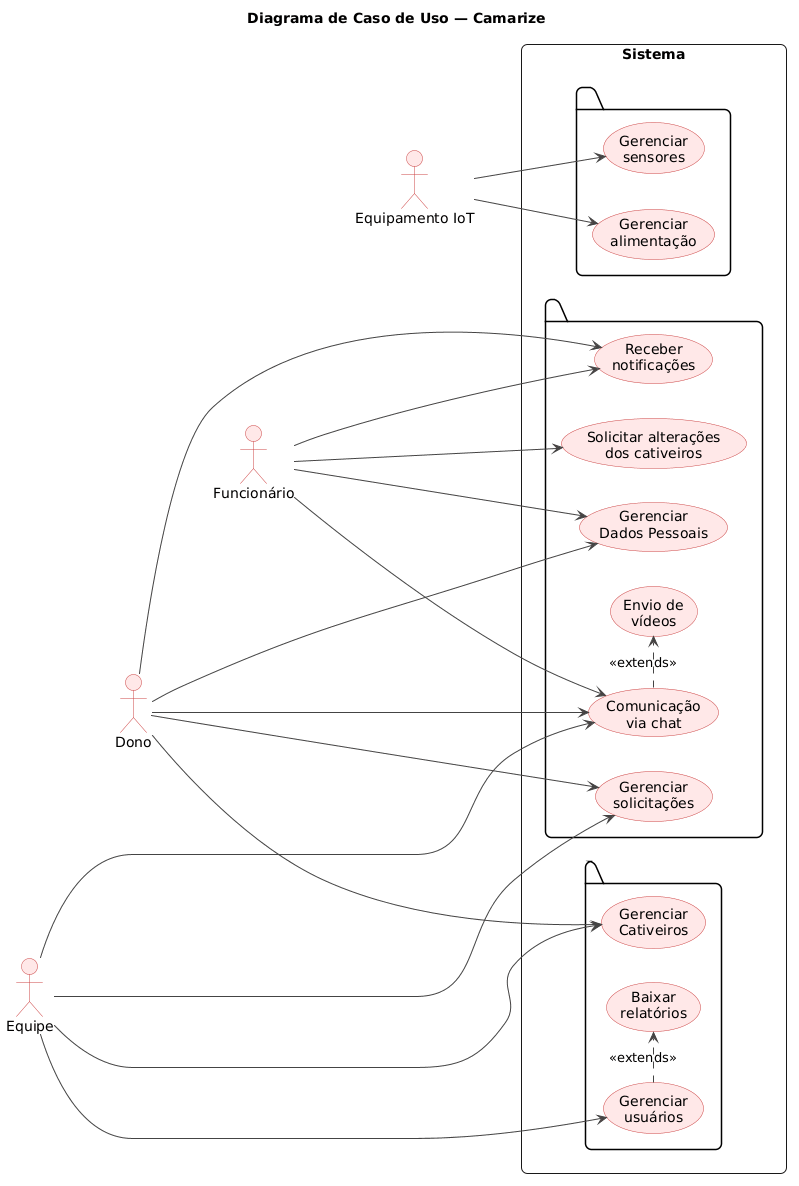
\includegraphics[width=0.8\textwidth]{imgs/diagrama_caso_uso.png}
    \\{\small Fonte: Autoria própria}
\end{figure}

\subsection{Diagrama de Classes}

Apresenta a estrutura orientada a objetos do sistema, com Users como classe central e seus relacionamentos com Cativeiros, Fazendas e os módulos de comunicação e notificações. Inclui os métodos de cada classe e as associações N:N por meio de coleções intermediárias.

\begin{figure}[H]
    \centering
    \caption{Diagrama de Classes}
    \label{fig:diagrama-classes}
        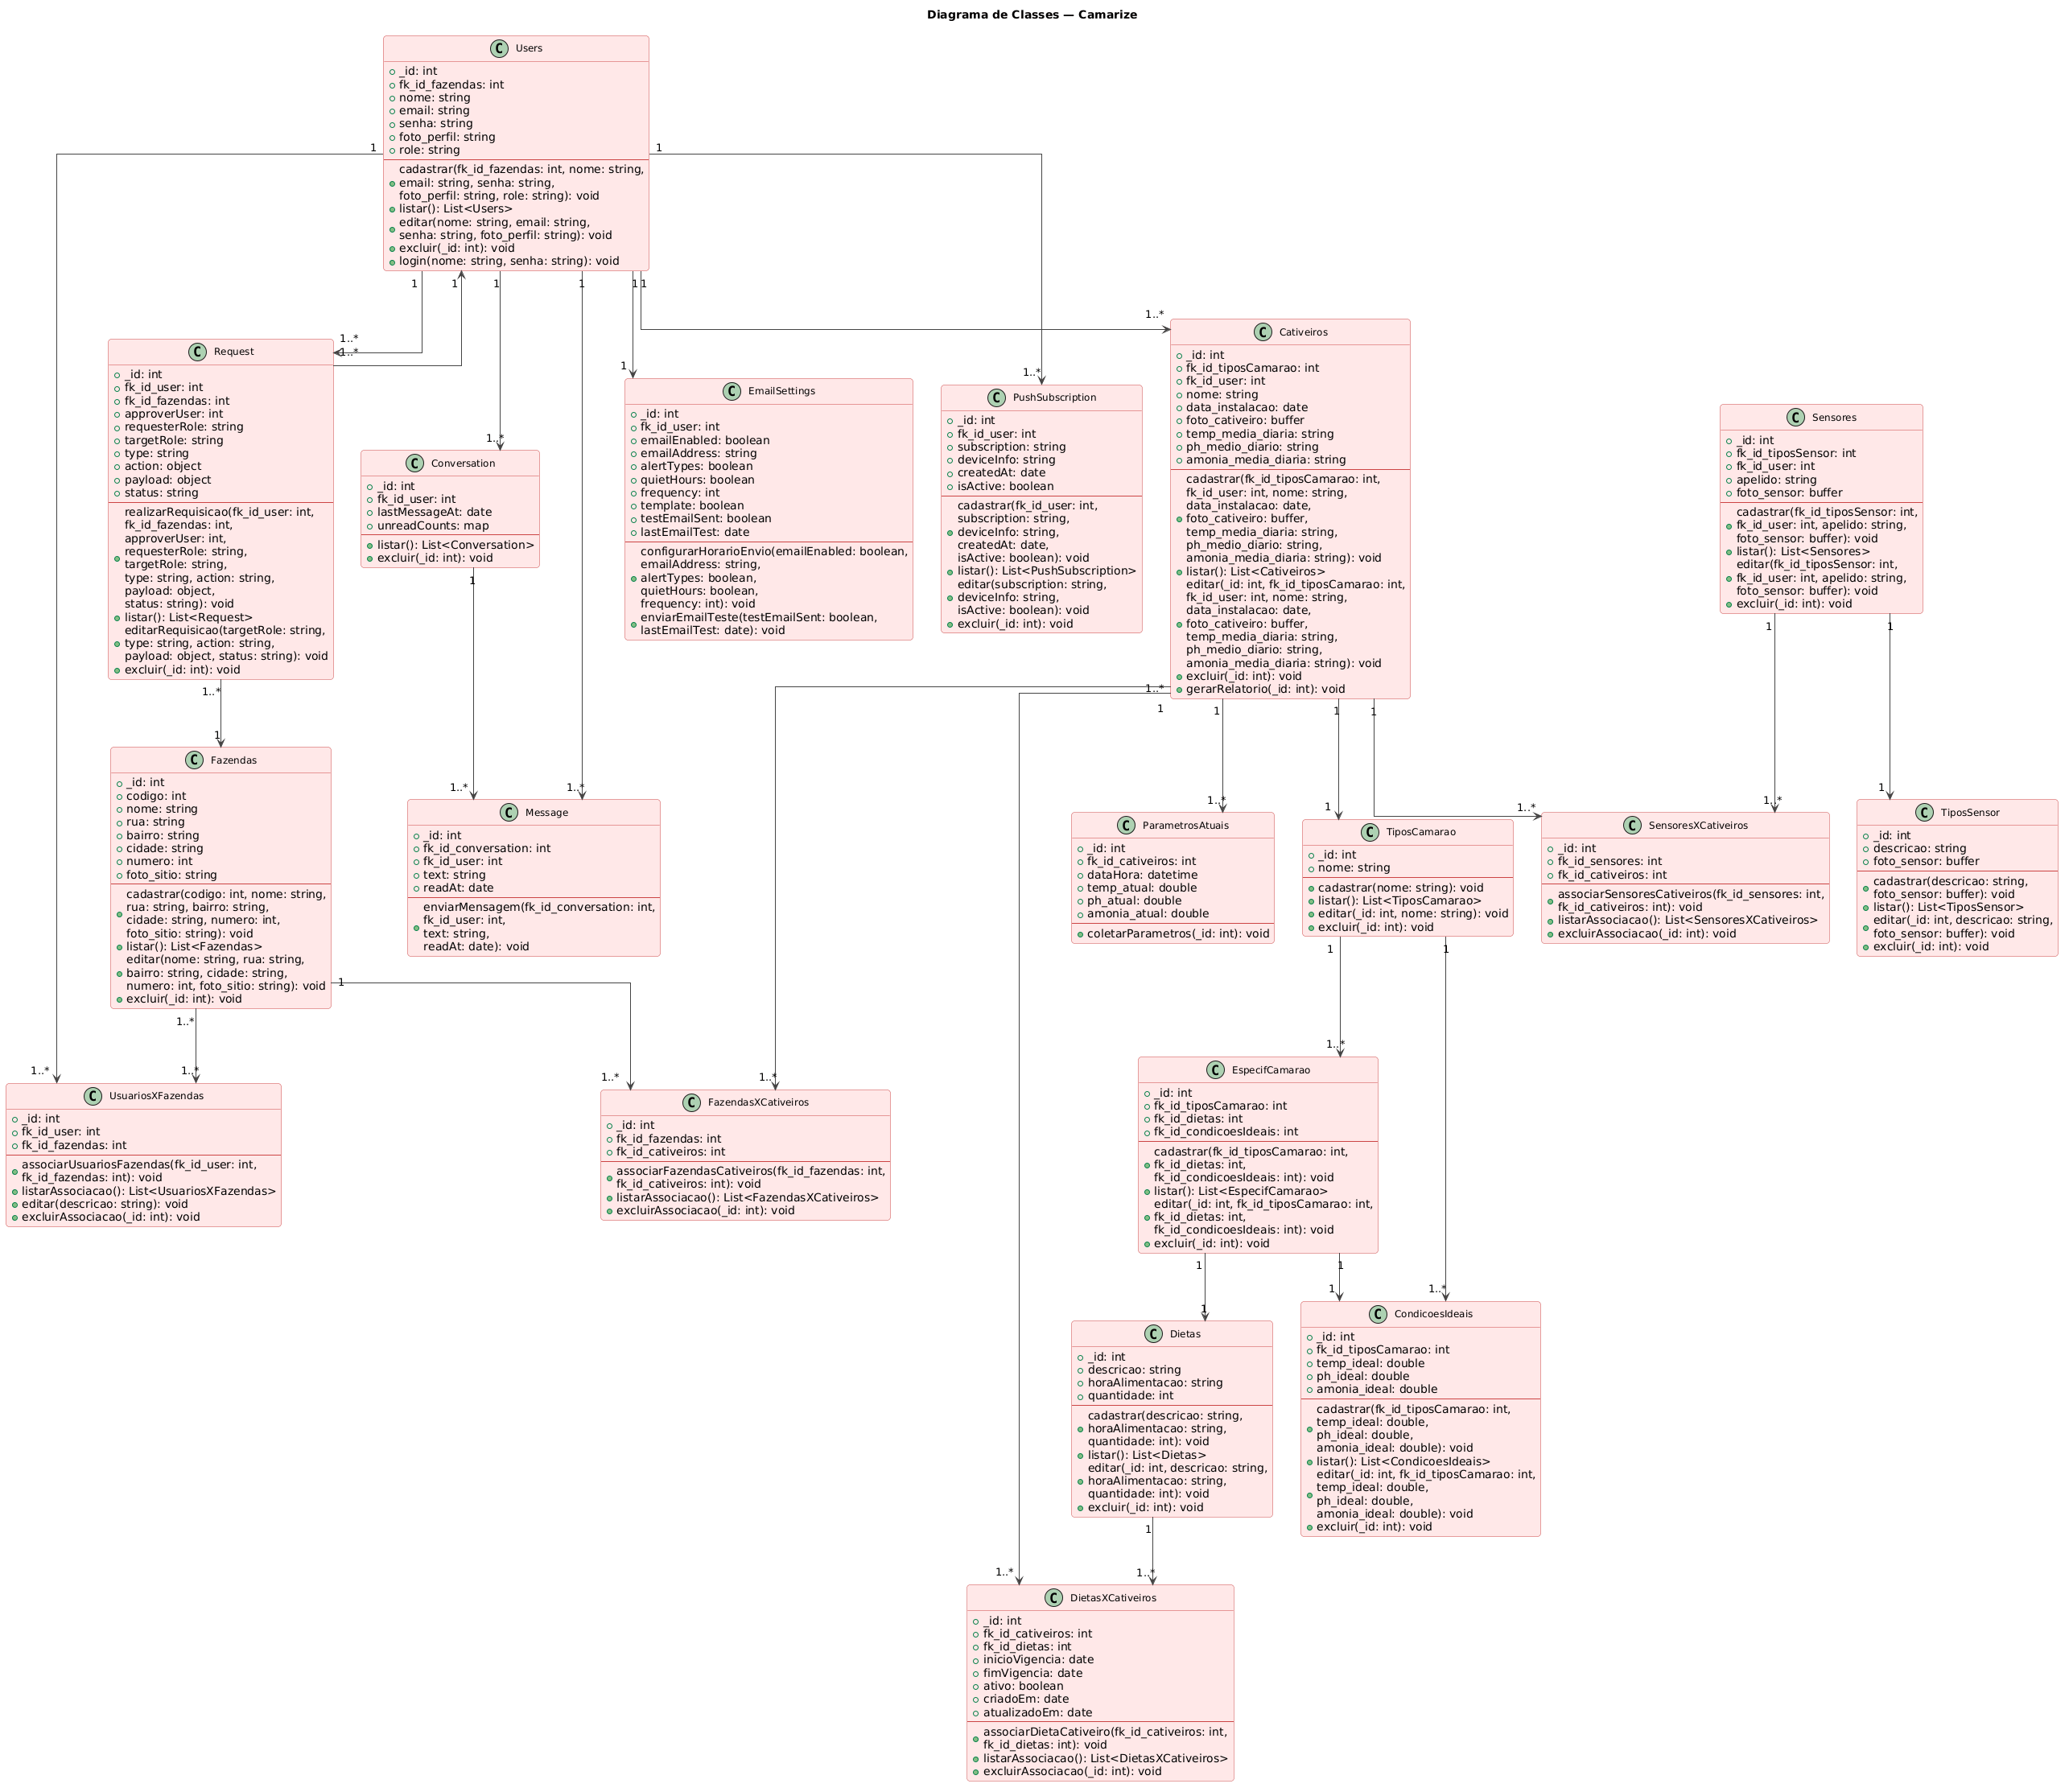
\includegraphics[width=1.1\textwidth]{imgs/diagrama_classes2.png}
    \\{\small Fonte: Autoria própria}
\end{figure}
\newpage

\subsection{Diagrama de Objetos}

O diagrama de objetos ilustra instâncias concretas das classes do sistema em um cenário de uso, exemplificando os valores dos atributos e os vínculos entre objetos em tempo de execução.

\begin{figure}[H]
    \centering
    \caption{Diagrama de Objetos}
    \label{fig:diagrama-objetos}
        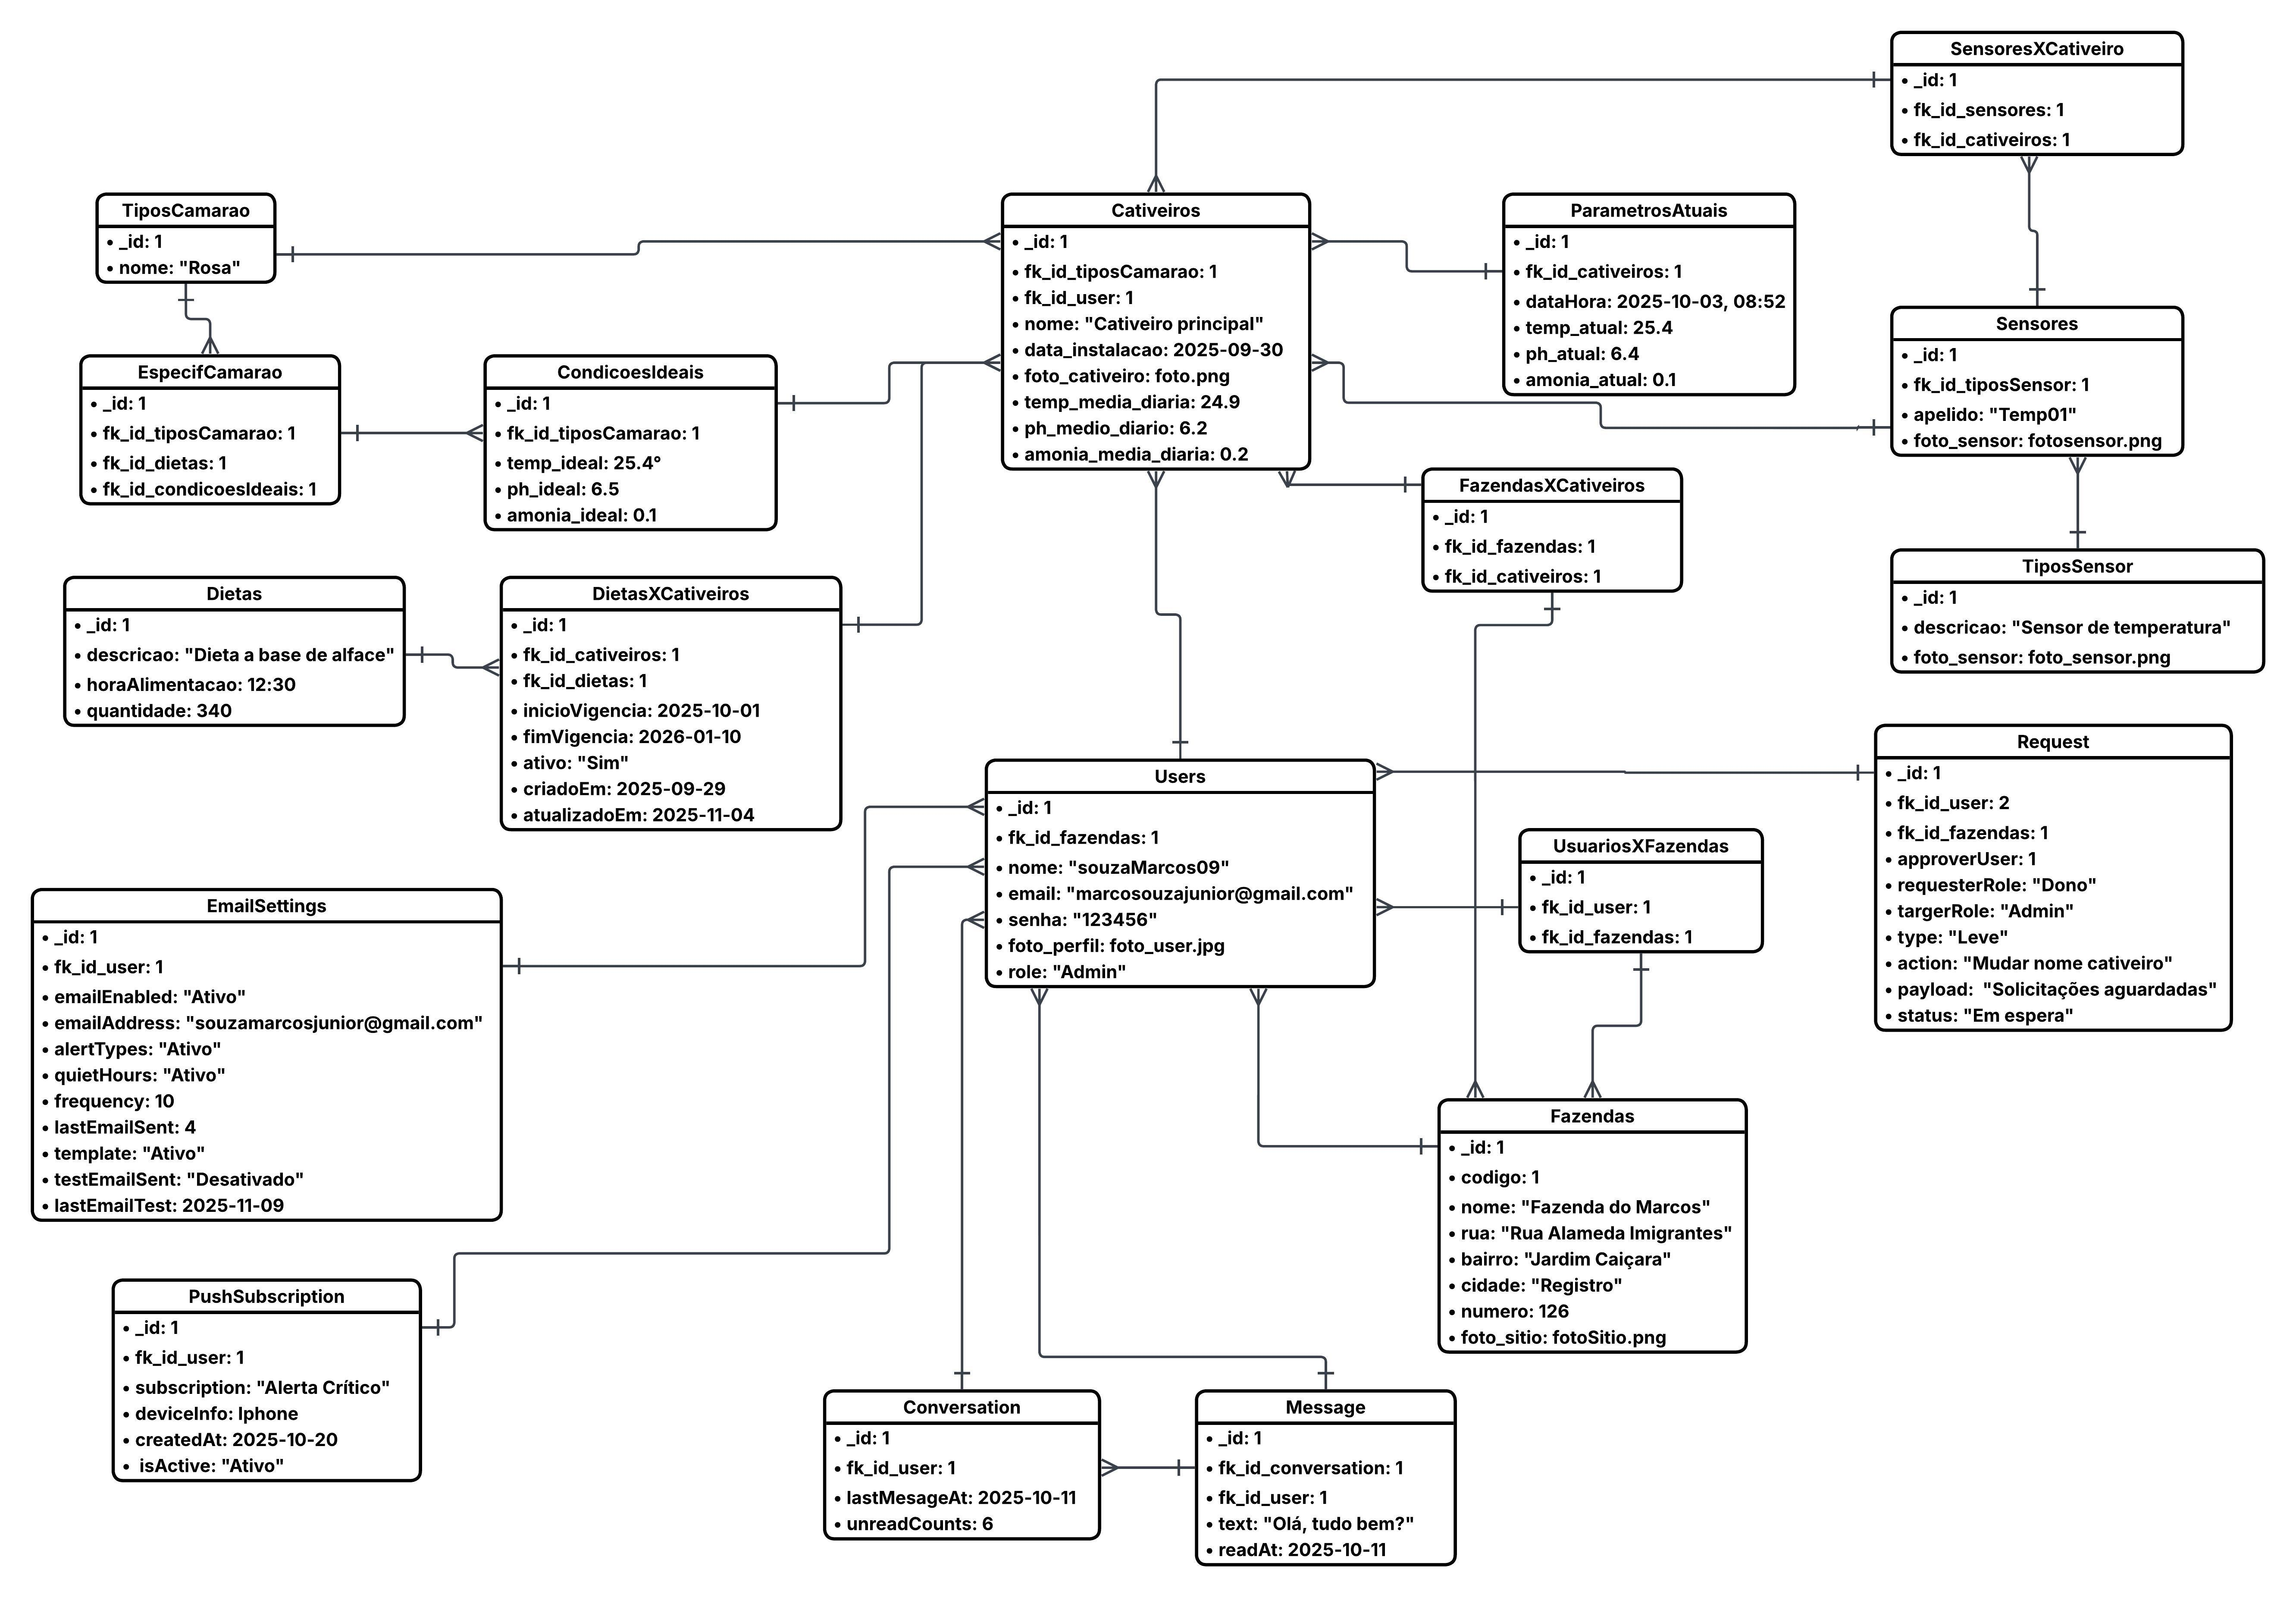
\includegraphics[width=1.0\textwidth]{imgs/diagrama_objetos.jpeg}
    \\{\small Fonte: Autoria própria}
\end{figure}

\subsection{Diagrama de Sequência}

Detalha três fluxos principais de interação: monitoramento em tempo real, visualização pelo usuário e controle de alimentação, envolvendo o Aplicativo, a API, o Banco de Dados e o ESP32.

\begin{figure}[H]
    \centering
    \caption{Diagrama de Sequência}
    \label{fig:diagrama-sequencia}
        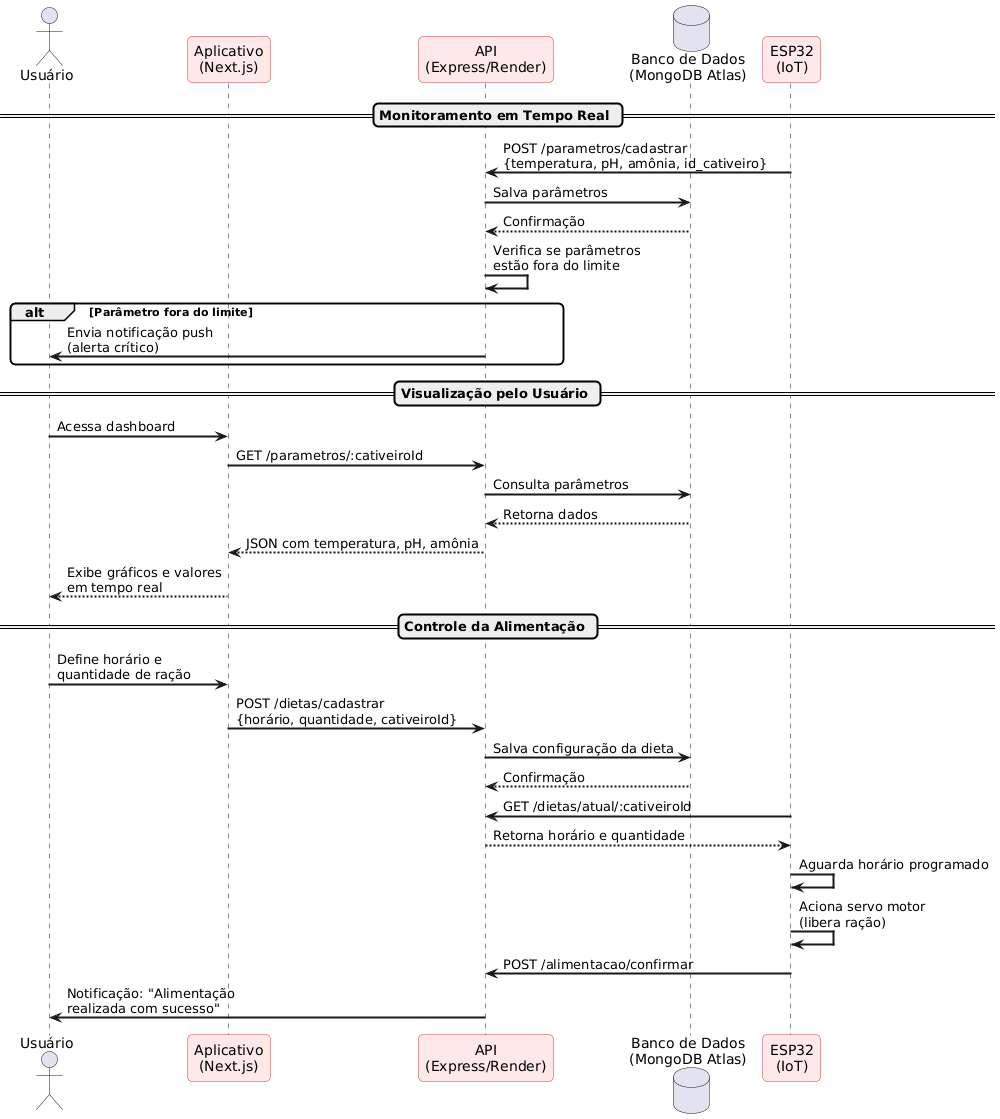
\includegraphics[width=\textwidth]{imgs/diagrama_sequencia.png}
    \\{\small Fonte: Autoria própria}
\end{figure}

\subsection{Diagrama de Atividades}

Descreve o fluxo completo de operação do sistema, desde o cadastro do usuário até o ciclo contínuo de monitoramento e controle de alimentação, incluindo a lógica de verificação de limites e envio de alertas.

\begin{figure}[H]
    \centering
    \caption{Diagrama de Atividades}
    \label{fig:diagrama-atividades}
        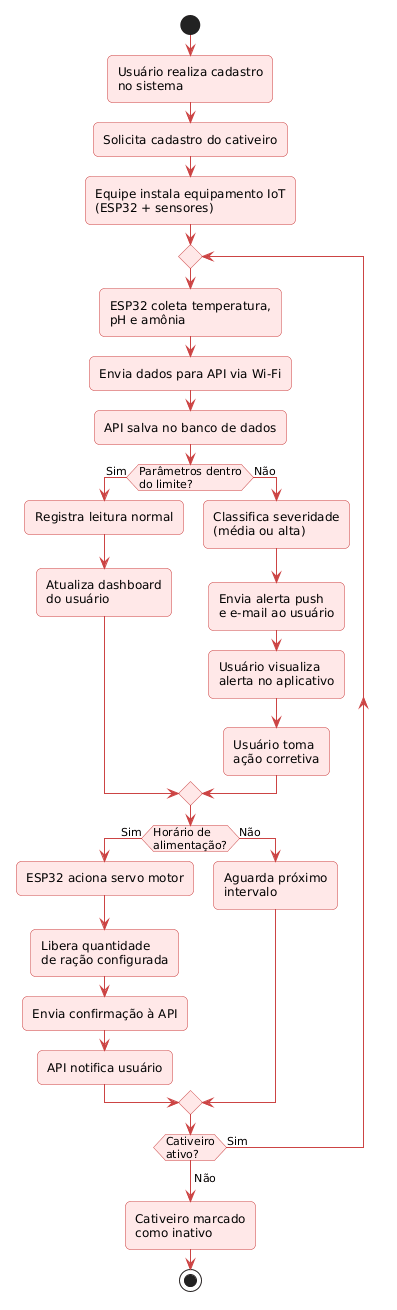
\includegraphics[width=0.4\textwidth]{imgs/diagrama_atividades.png}
    \\{\small Fonte: Autoria própria}
\end{figure}

\subsection{Diagrama de Componentes}

Organiza o sistema em três blocos principais: Frontend (Next.js/Vercel), Backend (Node.js + Express/Render) e Componente IoT (ESP32), com comunicação via HTTPS e conexão ao MongoDB Atlas via Mongoose.

\begin{figure}[H]
    \centering
    \caption{Diagrama de Componentes}
    \label{fig:diagrama-componentes}
        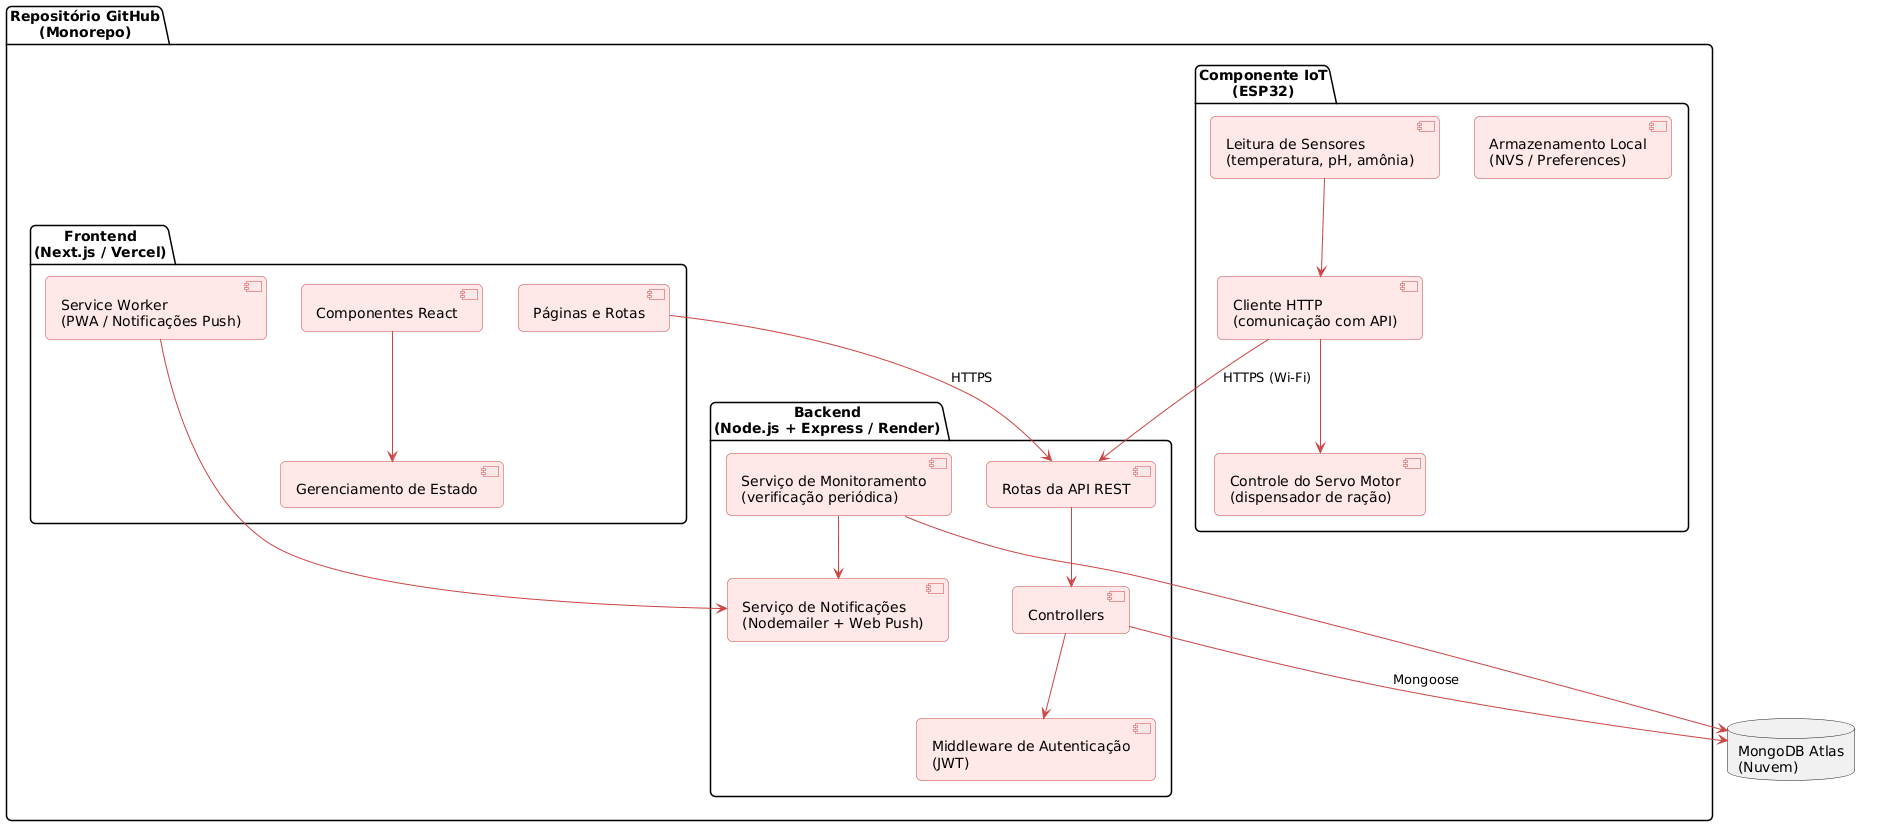
\includegraphics[width=\textwidth]{imgs/diagrama_componentes.png}
    \\{\small Fonte: Autoria própria}
\end{figure}

\subsection{Diagrama de Implantação}

Apresenta a distribuição física dos componentes em produção, incluindo a aplicação PWA na Vercel, a API REST no Render, o banco MongoDB Atlas e o ESP32 no ambiente do cativeiro, com \textit{deploy} contínuo via GitHub.

\begin{figure}[H]
    \centering
    \caption{Diagrama de Implantação}
    \label{fig:diagrama-implantacao}
        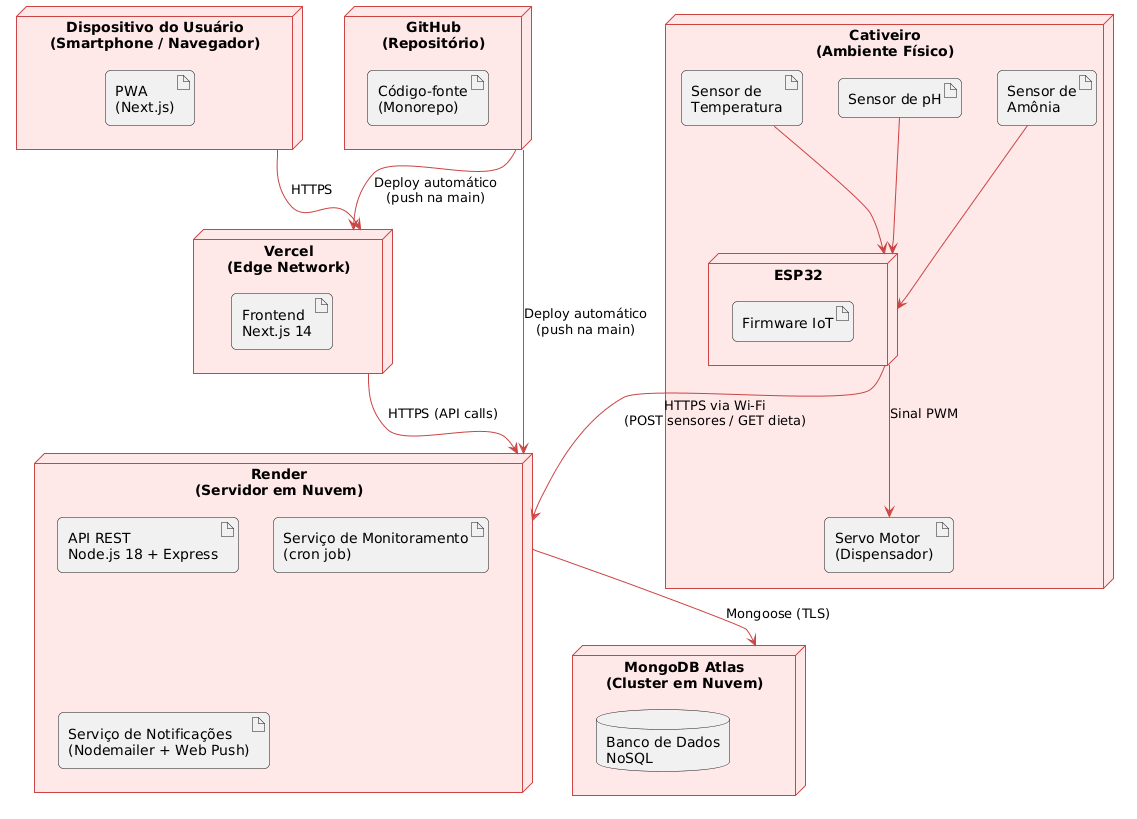
\includegraphics[width=0.8\textwidth]{imgs/diagrama_implantacao.png}
    \\{\small Fonte: Autoria própria}
\end{figure}

\subsection{Diagrama de Estados}

Modela o ciclo de vida de um cativeiro em quatro estados: AguardandoInstalação, Monitorando, EmAlerta e Inativo, com transições acionadas por eventos do sistema e ações do usuário.

\begin{figure}[H]
    \centering
    \caption{Diagrama de Estados}
    \label{fig:diagrama-estados}
        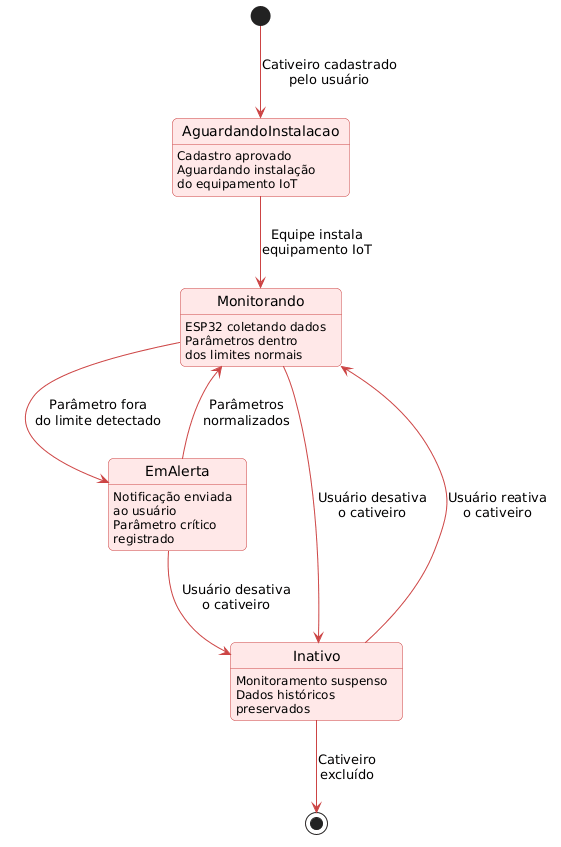
\includegraphics[width=0.8\textwidth]{imgs/diagrama_estados.png}
    \\{\small Fonte: Autoria própria}
\end{figure}

Para realizar a montagem dos diagramas, foi utilizada a ferramenta \textit{online} PlantUML, que permite a criação de diagramas UML através de código.

\section{Diagrama de Banco de Dados}

O diagrama de banco de dados representa a estrutura do banco de dados não relacional (NoSQL) utilizado no projeto, mostrando as coleções, seus campos e os relacionamentos entre elas.

\subsection{Modelo Conceitual}

O modelo conceitual representa as entidades e seus relacionamentos em alto nível, destacando as cardinalidades (1,1) e (1,N) entre todas as entidades do sistema de forma independente de tecnologia.

\begin{figure}[H]
    \centering
    \caption{Modelo Conceitual do Banco de Dados}
    \label{fig:modelo-conceitual}
        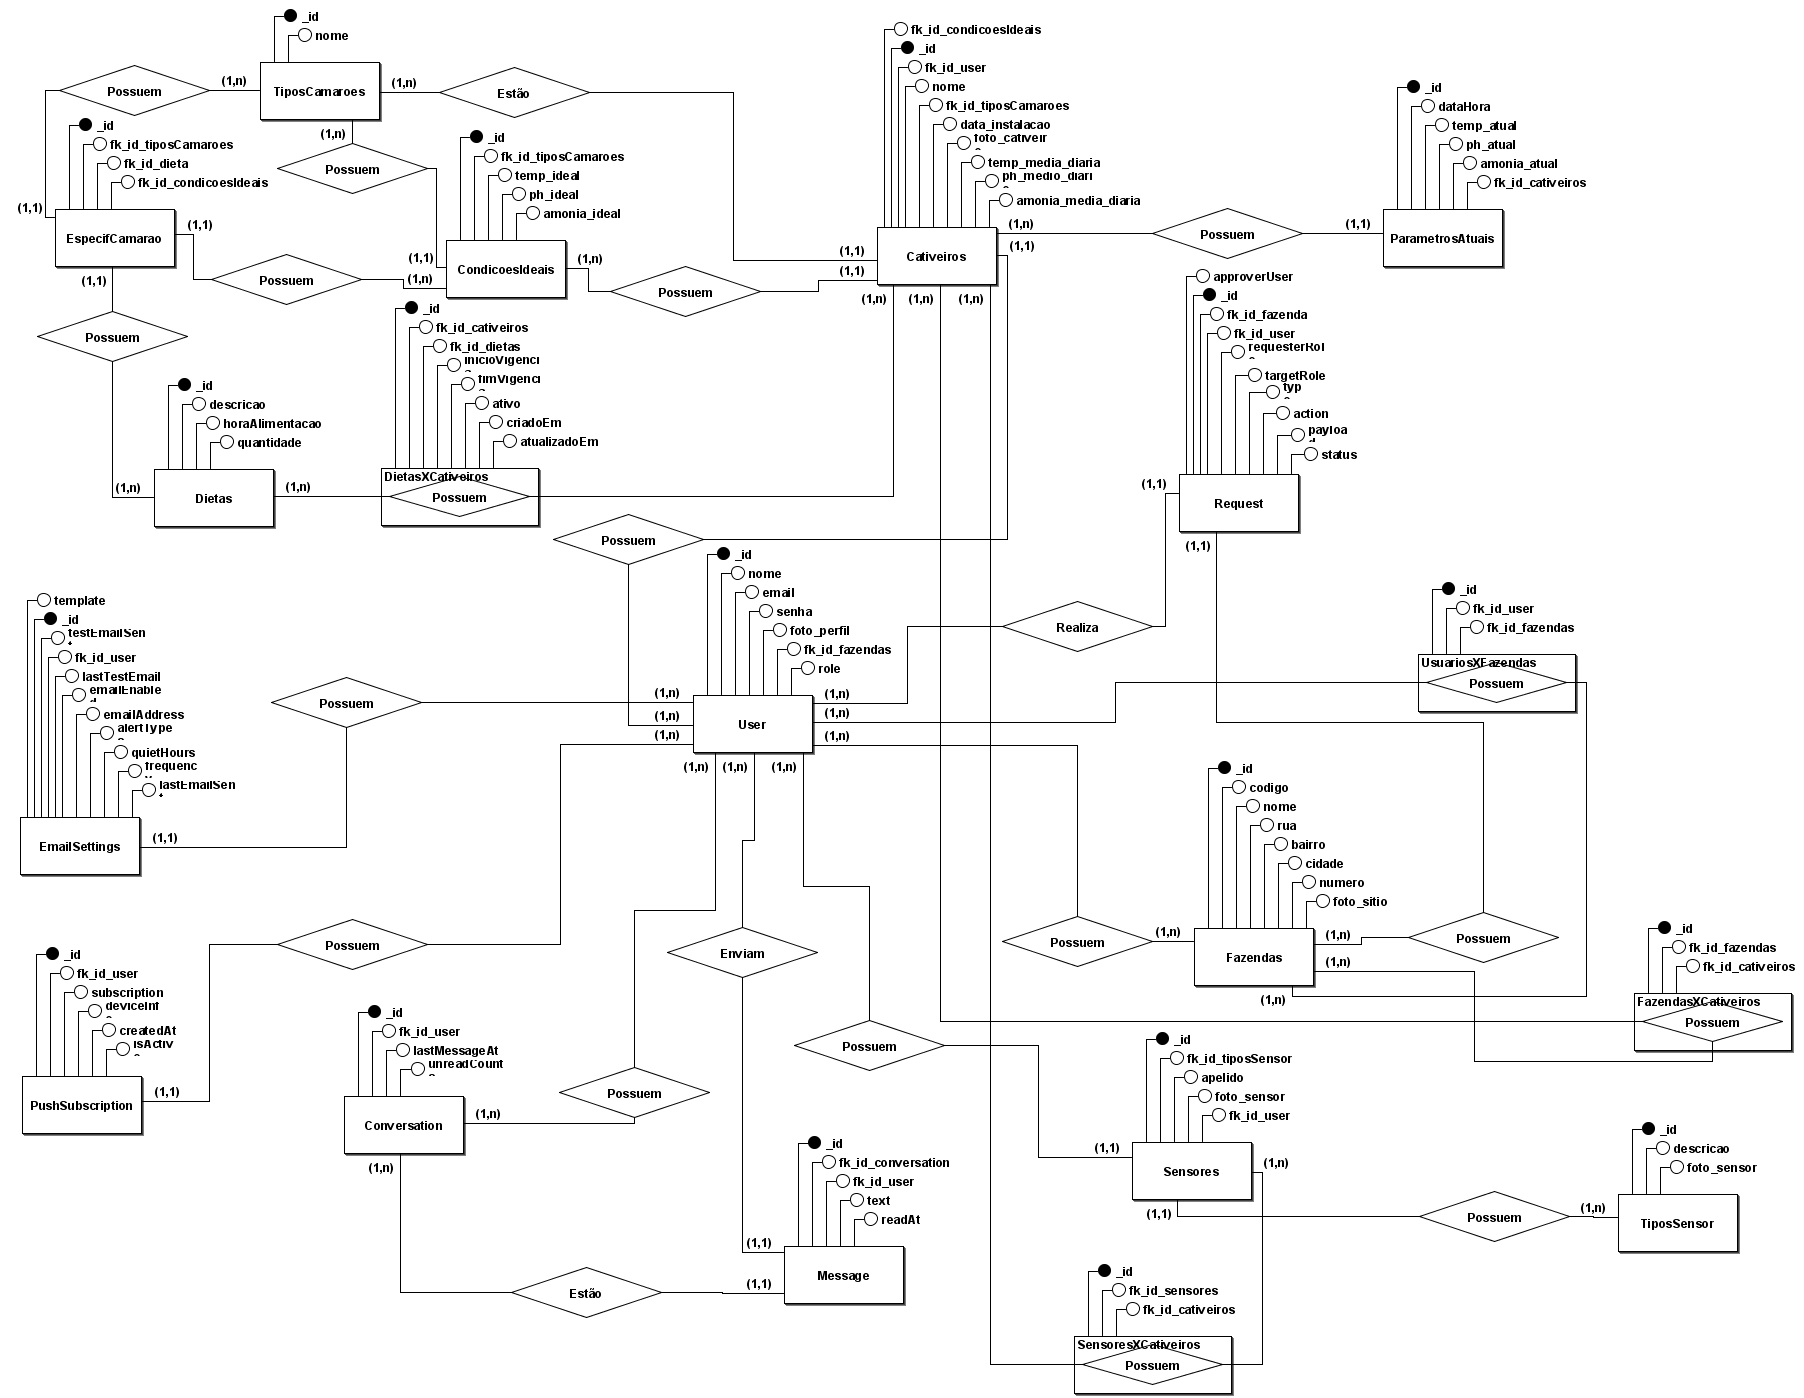
\includegraphics[width=1.1\textwidth]{imgs/modelo_conceitual.png}
    \\{\small Fonte: Autoria própria}
\end{figure}

\subsection{Modelo Lógico}

O modelo lógico refina o conceitual para um esquema de coleções MongoDB, detalhando os documentos como Tipos\_camarao, Cativeiros, Sitios, Parametros\_atuais, Dietas, Sensores, Usuarios, entre outros, com seus campos, tipos de dados e referências entre coleções.

\begin{figure}[H]
    \centering
    \caption{Modelo Lógico do Banco de Dados}
    \label{fig:modelo-logico}
        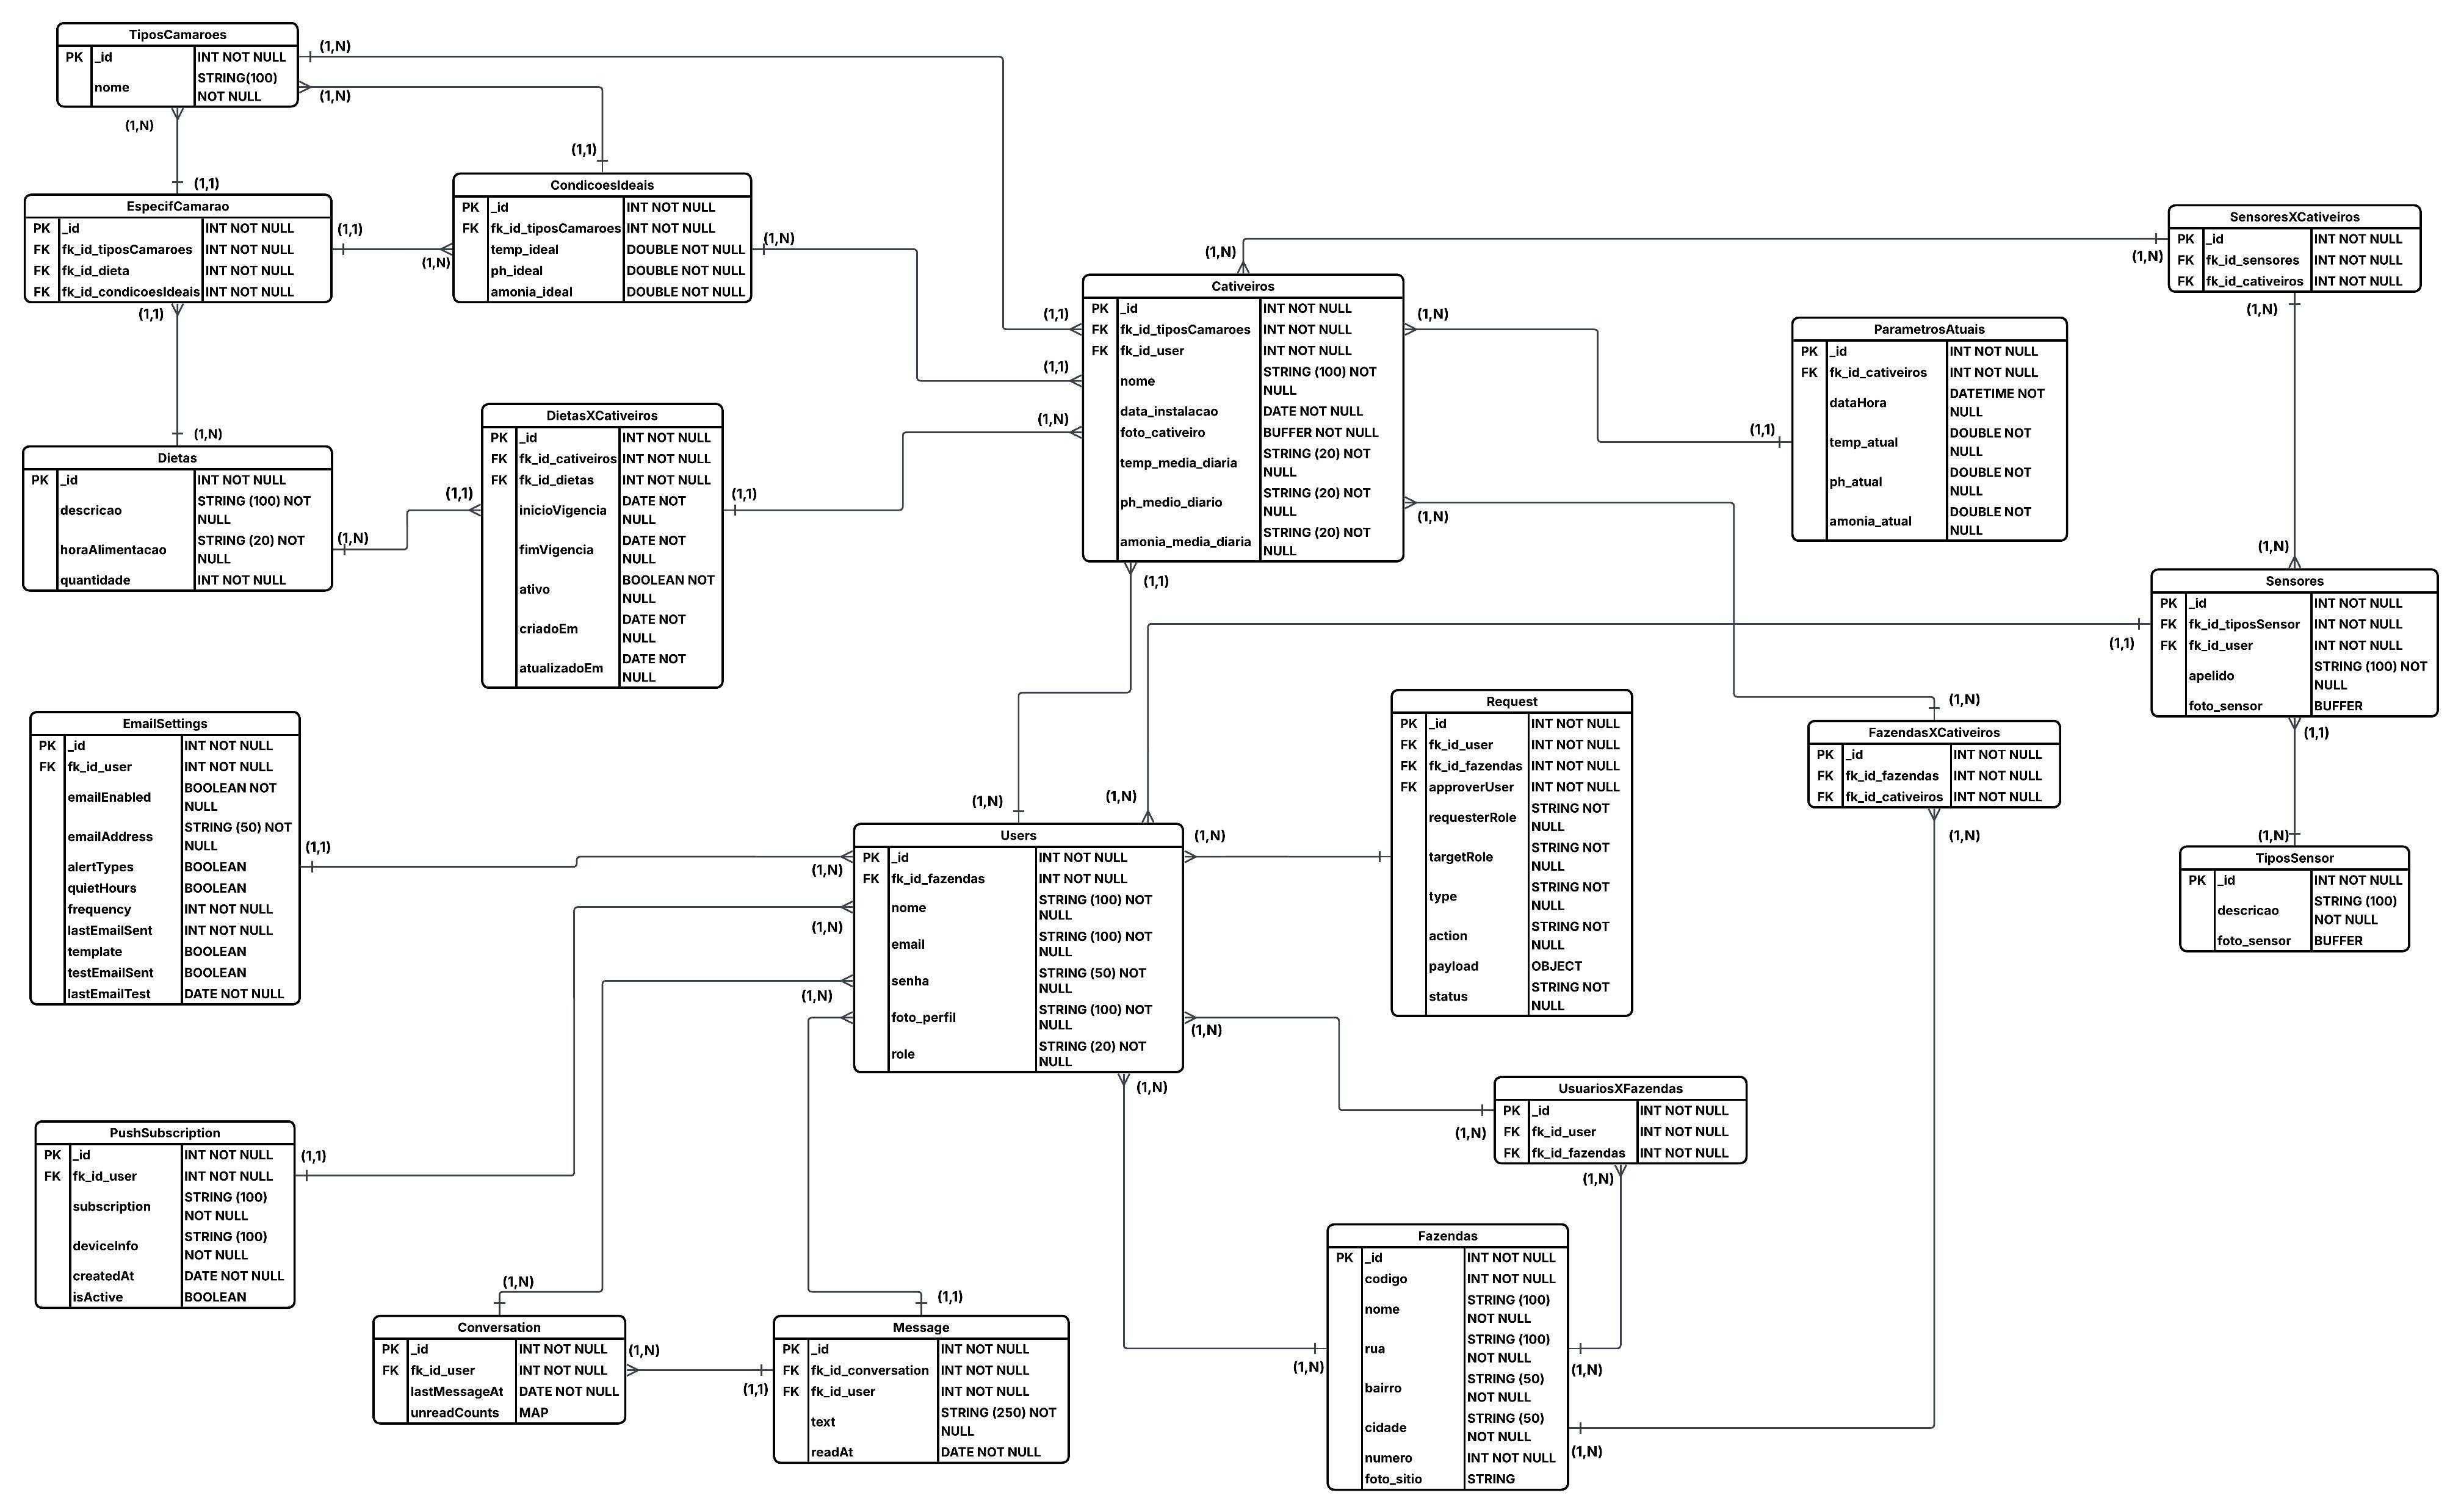
\includegraphics[width=1.1\textwidth]{imgs/modelo_logico.jpeg}
    \\{\small Fonte: Autoria própria}
\end{figure}

\subsection{Modelo Físico}

O modelo físico é a implementação final utilizando \textit{Mongoose Schemas}, com definições de tipos (String, Number, Boolean, Buffer, Map) e restrições (\texttt{required: true}), voltado para a criação direta das coleções no MongoDB Atlas, contemplando todas as entidades do sistema incluindo EmailSettings, PushSubscription, Conversation, Message e Request.

\begin{figure}[H]
    \centering
    \caption{Modelo Físico do Banco de Dados}
    \label{fig:modelo-fisico}
        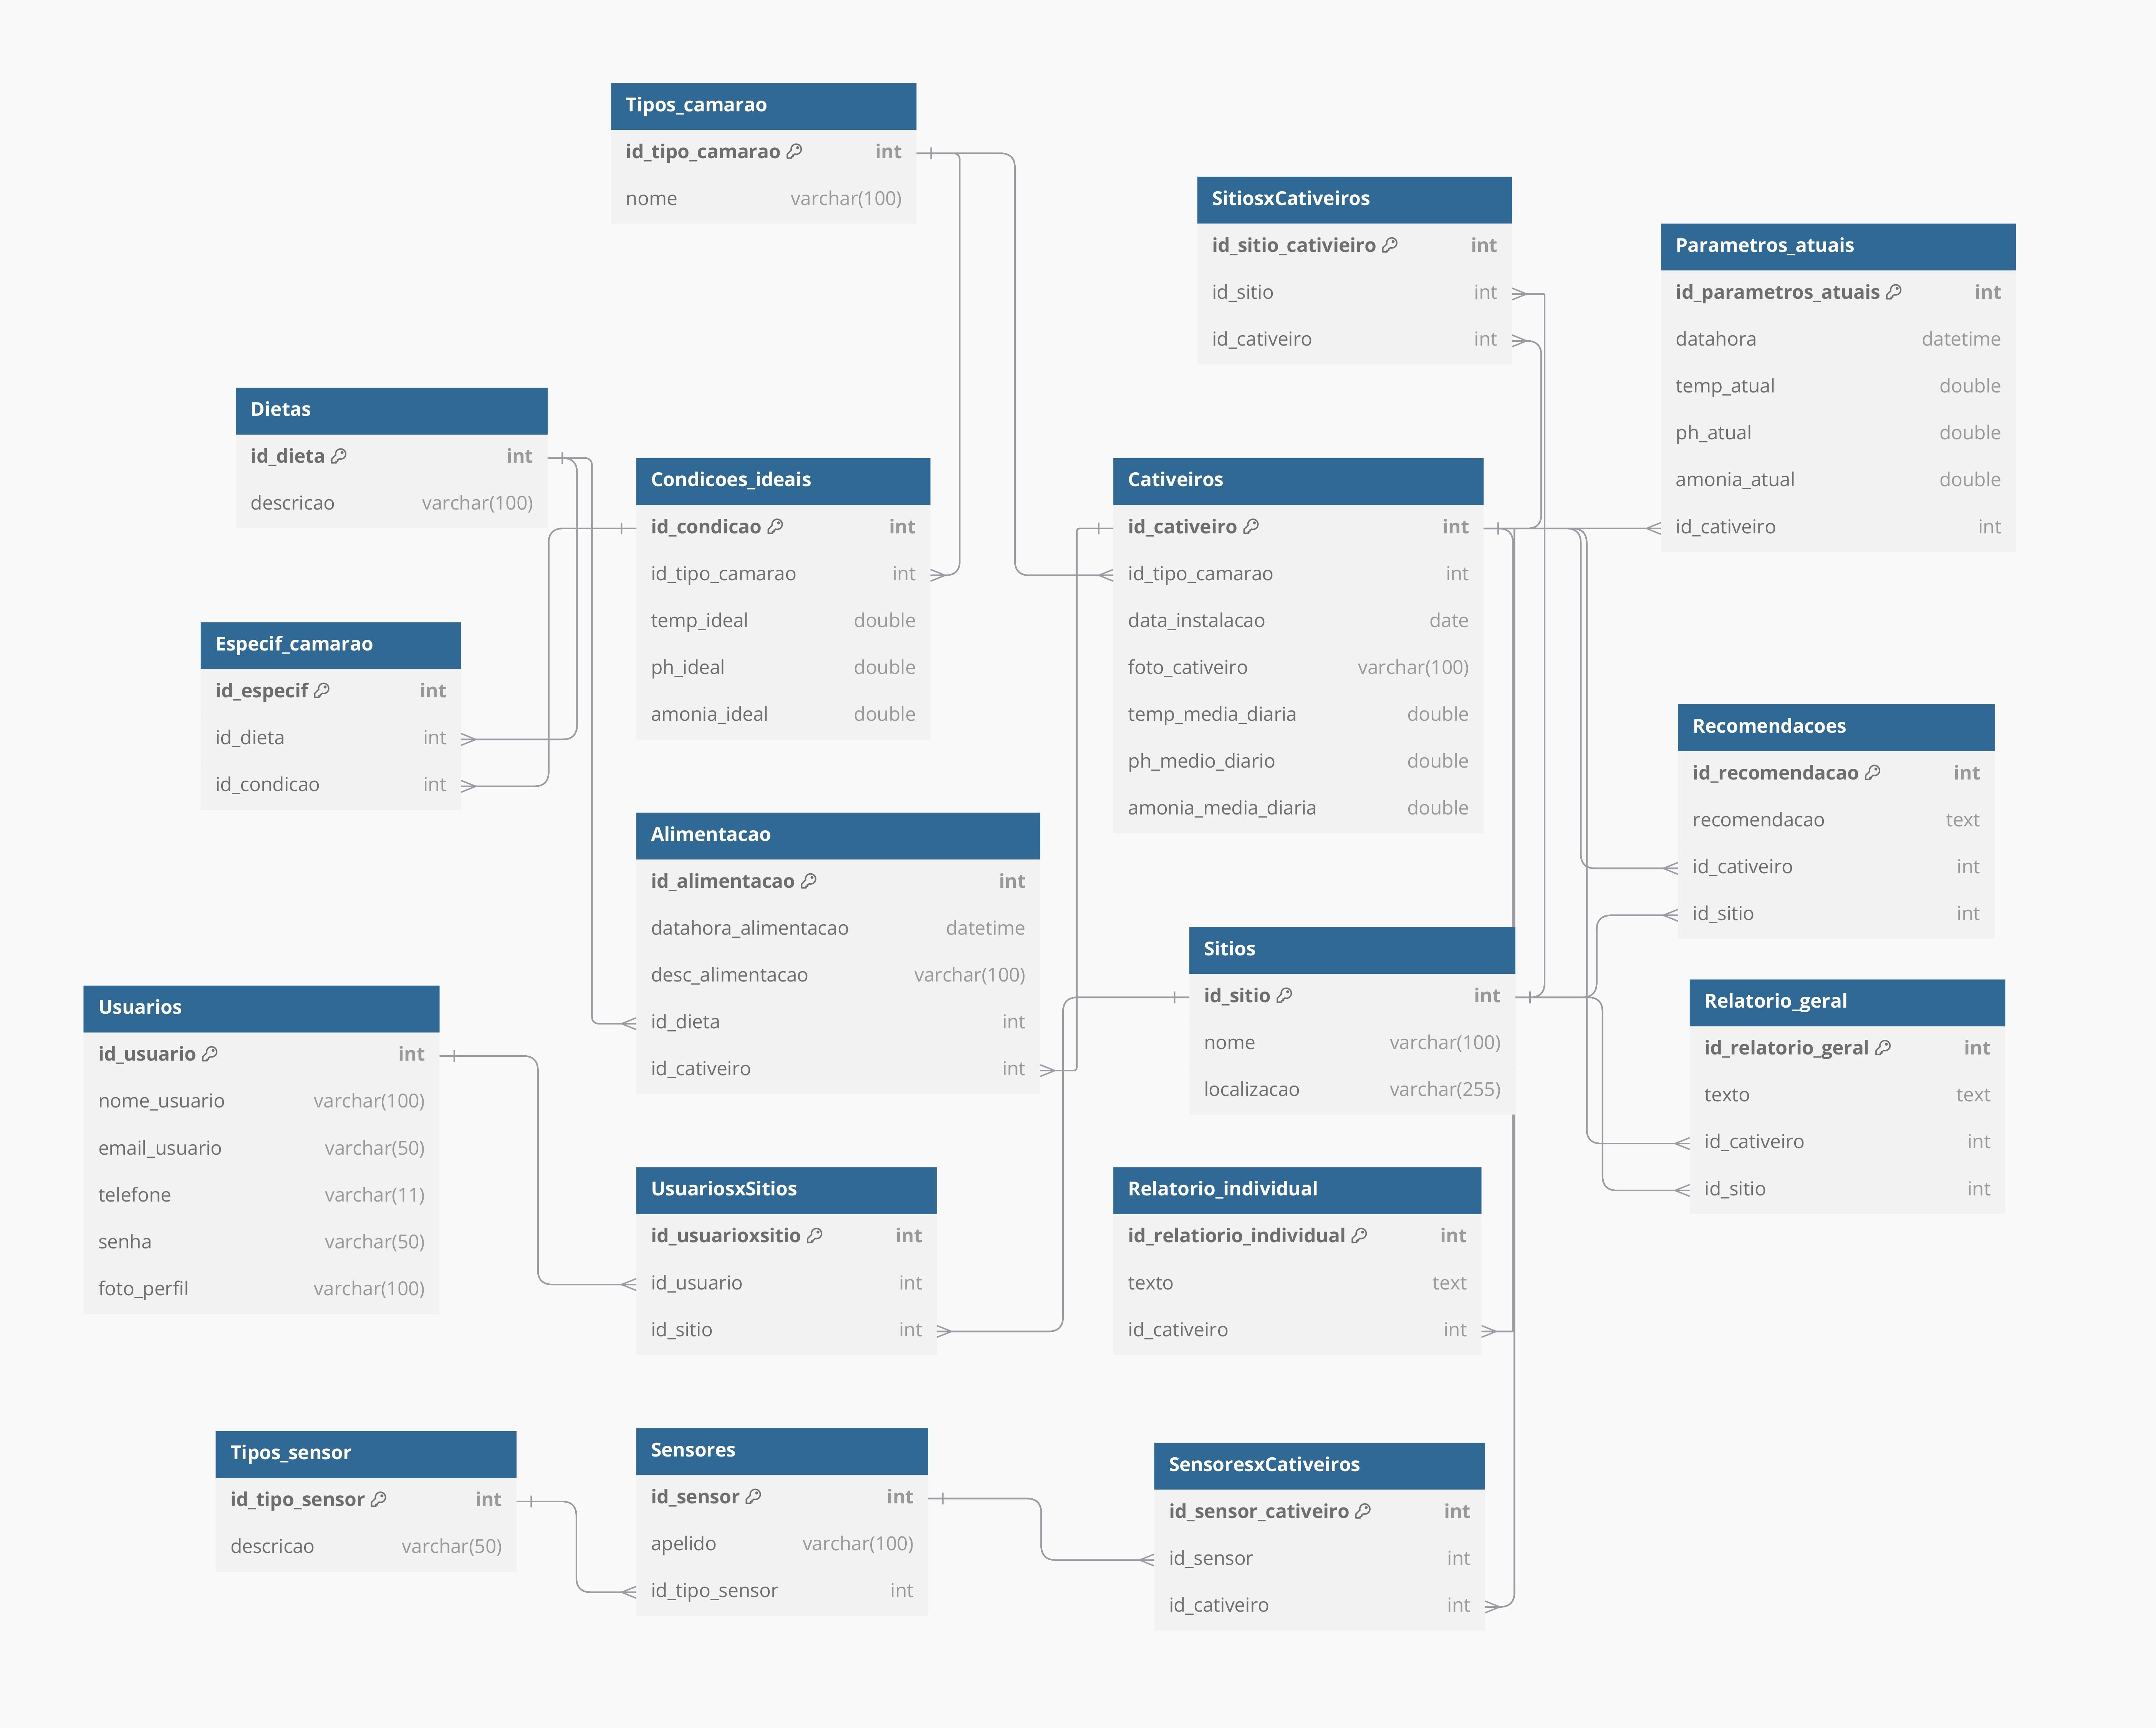
\includegraphics[width=1.1\textwidth]{imgs/modelo_fisico.jpg}
    \\{\small Fonte: Autoria própria}
\end{figure}

% ===== DEVOPS =====
\section{DevOps: Infraestrutura, Automação e Entrega Contínua}
DevOps \cite{kim2018} é uma cultura e conjunto de práticas que integra desenvolvimento de software (Dev) e operações de TI (Ops), focando em automação, colaboração e entrega contínua.\footnote{O termo "DevOps" foi popularizado por Patrick Debois em 2009.}

\subsection{Pipeline CI/CD}
O pipeline de integração contínua é executado automaticamente a cada push na branch \texttt{main}, garantindo a qualidade do código:
\begin{figure}[H]
\centering
\begin{tikzpicture}[
    node distance=1.5cm,
    every node/.style={rectangle, draw, rounded corners, 
                       fill=secondarycolor!20, 
                       text width=2cm, 
                       align=center,
                       font=\small,
                       minimum height=1cm}
]
\node (code) {Code};
\node (build) [right of=code, xshift=1cm] {Build};
\node (test) [right of=build, xshift=1cm] {Test};
\node (deploy) [right of=test, xshift=1cm] {Deploy};
\draw[->, thick] (code) -- (build);
\draw[->, thick] (build) -- (test);
\draw[->, thick] (test) -- (deploy);
\draw[->, thick, dashed] (deploy) to[bend right=45] (code);
\end{tikzpicture}
\caption{Pipeline CI/CD}
\label{fig:cicd}
\end{figure}

\subsection{Configuração CI/CD}
O pipeline é composto por dois jobs paralelos: build do frontend (Next.js) e verificação de sintaxe da API (Node.js). Além disso, a Vercel realiza deploy automático do frontend a cada push:
\begin{verbatim}
name: CI
on:
  push:
    branches: [main]
jobs:
  build-frontend:
    name: Frontend build
    runs-on: ubuntu-latest
    defaults:
      run:
        working-directory: front-react
    steps:
      - uses: actions/checkout@v4
      - uses: actions/setup-node@v4
        with:
          node-version: 18
          cache: npm
          cache-dependency-path: front-react/package-lock.json
      - run: npm ci
      - run: npm run build
  check-api:
    name: API syntax check
    runs-on: ubuntu-latest
    steps:
      - uses: actions/checkout@v4
      - uses: actions/setup-node@v4
        with:
          node-version: 18
      - run: find api -name "*.js" -not -path "*/node_modules/*"
             -exec node --check {} \;
\end{verbatim}

\subsection{Infraestrutura como Código}
\begin{table}[H]
\centering
\caption{Ferramentas DevOps Utilizadas}
\label{tab:devops-tools}
\begin{tabular}{|l|l|p{6cm}|}
\hline
\textbf{Categoria} & \textbf{Ferramenta} & \textbf{Finalidade} \\
\hline
Controle de Versão & Git + GitHub & Versionamento de código e colaboração \\
CI/CD & GitHub Actions & Automação de build e verificação de sintaxe \\
Hosting Frontend & Vercel & Hospedagem e deploy automático do Next.js \\
Hosting Backend & Render & Hospedagem da API Express em produção \\
Containerização & Docker + Compose & Empacotamento e orquestração local de serviços \\
Banco de Dados & MongoDB Atlas & Banco de dados NoSQL em nuvem (cluster gerenciado) \\
Documentação API & Swagger UI & Documentação interativa de endpoints REST \\
Tunelamento & Ngrok & Exposição de serviços locais para testes externos \\
\hline
\end{tabular}
\end{table}


\subsection{Infraestrutura do Sistema}
Esta seção documenta como o sistema funciona em diferentes ambientes e plataformas.
\subsubsection{Arquitetura de Rede}
\begin{table}[H]
\centering
\caption{Componentes de Infraestrutura}
\label{tab:infrastructure}
\begin{tabular}{|l|p{10cm}|}
\hline
\textbf{Componente} & \textbf{Descrição} \\
\hline
\textbf{Rede Local (LAN)} & 
\begin{itemize}[leftmargin=*, nosep]
    \item Ambiente local para desenvolvimento e testes da aplicação
    \item Docker Compose para integração entre API (porta 4000) e Frontend (porta 3000)
    \item Comunicação entre serviços via \texttt{localhost} com portas dedicadas
    \item Controle de versão integrado ao Git e GitHub
    \item Testes de sintaxe e build executados via CI antes do merge
\end{itemize} \\
\hline
\textbf{Cloud (Nuvem)} & 
\begin{itemize}[leftmargin=*, nosep]
    \item Frontend hospedado na Vercel com deploy automático via integração GitHub
    \item Backend hospedado no Render como serviço web
    \item Banco de dados MongoDB Atlas em nuvem (cluster gerenciado)
    \item Deploy automático do frontend a cada push na branch \texttt{main}
    \item Replicação e backup automático fornecidos pelo MongoDB Atlas
    \item Variáveis de ambiente gerenciadas nas plataformas Vercel e Render
\end{itemize} \\
\hline
\textbf{Dispositivos Móveis} & 
\begin{itemize}[leftmargin=*, nosep]
    \item Interface responsiva (PWA) adaptada para smartphones e tablets
    \item Service Worker para cache offline e notificações push
    \item Compatibilidade com navegadores móveis modernos (Chrome, Safari)
    \item Push Notifications via Web Push API (VAPID)
    \item Suporte para iOS e Android via navegador
\end{itemize} \\
\hline
\textbf{Segurança} & 
\begin{itemize}[leftmargin=*, nosep]
    \item SSL/TLS fornecido automaticamente pela Vercel e pelo Render
    \item Autenticação via JSON Web Tokens (JWT) com validação de \texttt{tokenVersion}
    \item Senhas criptografadas com bcrypt (migração transparente de senhas legadas)
    \item CORS configurado para origens permitidas
    \item Controle de acesso por roles (\texttt{master}, \texttt{admin}, \texttt{membro})
    \item Middleware de bloqueio de escrita para membros (\texttt{BlockMembersWrite})
\end{itemize} \\
\hline
\end{tabular}
\end{table}

\subsubsection{Diagrama de Infraestrutura}

Para ilustrar como os componentes se conectam:

\begin{figure}[H]
\centering
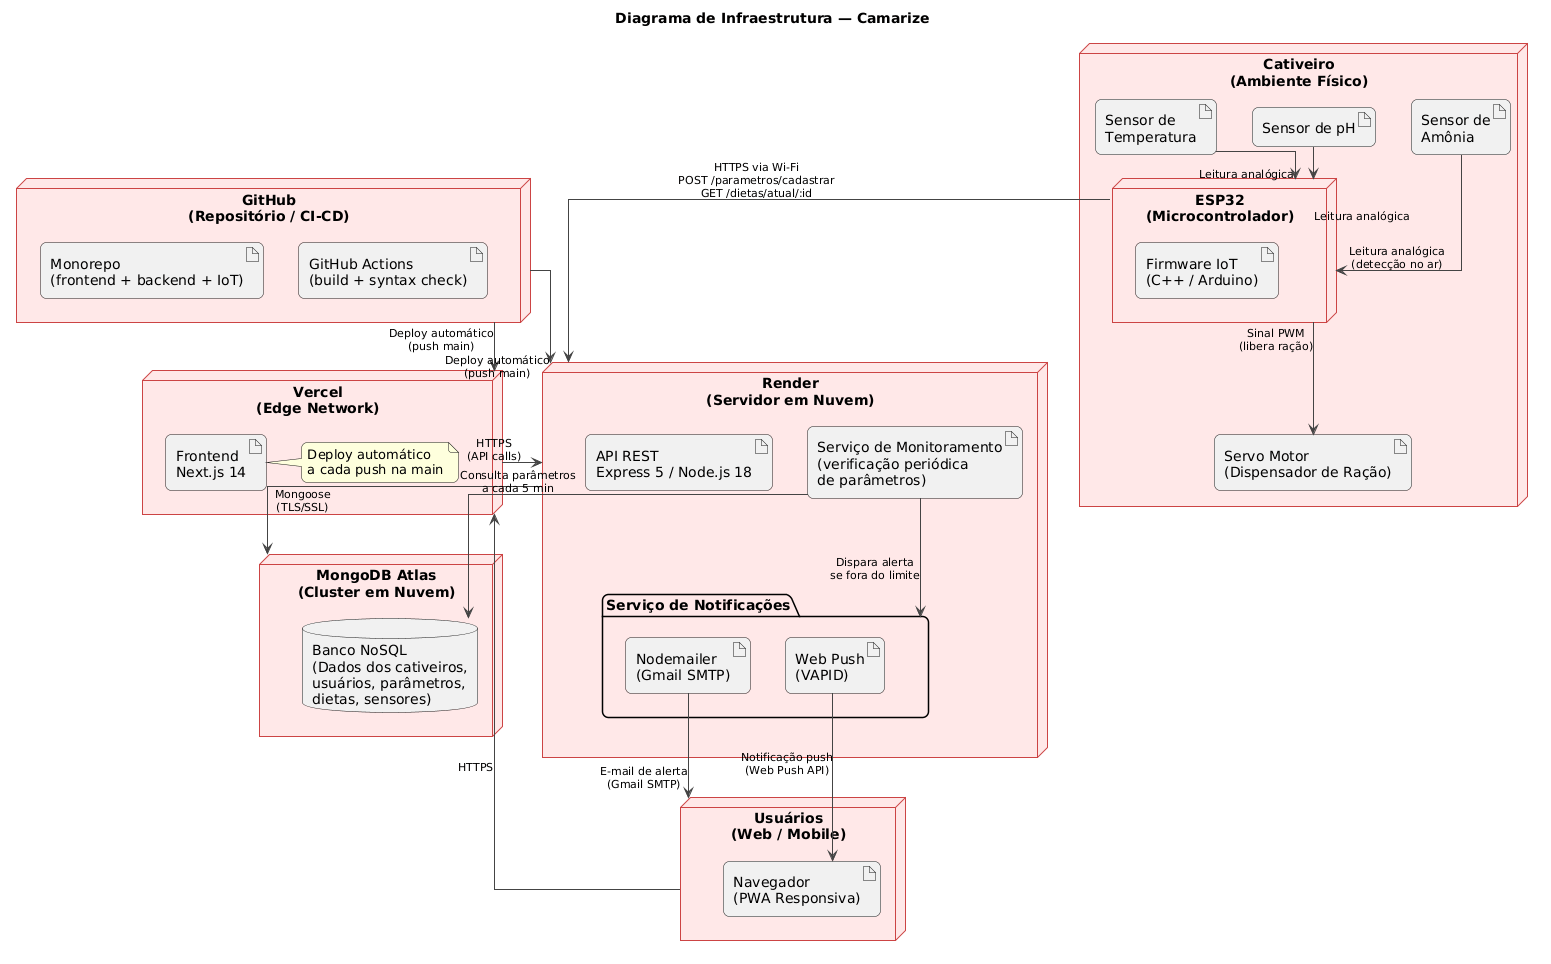
\includegraphics[width=\textwidth]{imgs/diagrama_infraestrutura.png}
\caption{Diagrama de Infraestrutura do Sistema}
\label{fig:infrastructure-diagram}
\end{figure}


\begin{itemize}
    \item \textbf{Usuários Web/Mobile:} Acessam via navegador através de HTTPS (PWA responsiva)
    \item \textbf{Frontend:} Next.js 14 hospedado na Vercel (deploy automático)
    \item \textbf{Backend:} API Express 5 hospedada no Render (Node.js 18)
    \item \textbf{Banco de Dados:} MongoDB Atlas (cluster em nuvem)
    \item \textbf{Monitoramento:} Serviço interno com verificação periódica de parâmetros dos cativeiros
    \item \textbf{Notificações:} Nodemailer (Gmail SMTP) para alertas por e-mail + Web Push para notificações no navegador
    \item \textbf{ESP32:} Sensores IoT enviando dados de temperatura, pH e amônia via API REST
\end{itemize}

\subsection{Arquitetura de Deploy}
A arquitetura de deployment em produção utiliza serviços gerenciados na nuvem:
\begin{figure}[H]
\centering
\begin{tikzpicture}[
    node distance=2cm,
    component/.style={rectangle, draw, rounded corners, 
                      fill=secondarycolor!20, 
                      text width=3cm, 
                      align=center,
                      minimum height=1.2cm}
]
\node[component] (user) {Usuário\\(Browser/PWA)};
\node[component, below left of=user, xshift=-2cm, yshift=-1cm] (vercel) {Vercel\\(Frontend)};
\node[component, below right of=user, xshift=2cm, yshift=-1cm] (render) {Render\\(API Backend)};
\node[component, below of=render, yshift=-1.5cm] (mongo) {MongoDB Atlas\\(Banco de Dados)};
\node[component, below of=vercel, yshift=-1.5cm] (github) {GitHub\\(Repositório)};
\draw[->, thick] (user) -- (vercel);
\draw[->, thick] (user) -- (render);
\draw[<->, thick] (vercel) -- node[above, font=\scriptsize] {API calls} (render);
\draw[<->, thick] (render) -- (mongo);
\draw[->, thick, dashed] (github) -- node[left, font=\scriptsize] {deploy} (vercel);
\draw[->, thick, dashed] (github) -- node[right, font=\scriptsize] {deploy} (render);
\end{tikzpicture}
\caption{Arquitetura de Deployment em Produção}
\label{fig:deployment}
\end{figure}

\subsection{Configuração Docker Compose (Desenvolvimento)}
Para o ambiente de desenvolvimento local, utiliza-se Docker Compose para orquestrar os serviços. Em produção, o sistema é hospedado diretamente nas plataformas Vercel (\textit{frontend}) e Render (API), sem utilização de containers:
\begin{verbatim}
services:
  api:
    build: ../api
    container_name: camarize-api
    restart: unless-stopped
    env_file: ../api/.env
    environment:
      - NODE_ENV=development
      - PORT=4000
    ports:
      - "4000:4000"
  frontend:
    build: ../front-react
    container_name: camarize-frontend
    restart: unless-stopped
    environment:
      - NEXT_PUBLIC_API_URL=http://localhost:4000
      - NEXT_PUBLIC_SSE_URL=http://localhost:4000
    depends_on:
      - api
    ports:
      - "3000:3000"
\end{verbatim}

\subsection{Monitoramento e Alertas}
O sistema possui um serviço de monitoramento automático que verifica periodicamente os parâmetros dos cativeiros:
\begin{itemize}
    \item \textbf{Intervalo de Verificação:} Configurável via variável de ambiente (\texttt{MONITORING\_INTERVAL\_MINUTES}, padrão: 5 minutos)
    \item \textbf{Parâmetros Monitorados:} Temperatura, pH e Amônia
    \item \textbf{Tolerâncias:} Temperatura (15\%), pH (20\%), Amônia (25\%)
    \item \textbf{Severidade:} Classificação automática em \texttt{media} ou \texttt{alta}
    \item \textbf{Canais de Alerta:} E-mail (Gmail SMTP via Nodemailer) com respeito a quiet hours e rate limiting
    \item \textbf{Health Check:} Endpoint \texttt{/api/health} para verificação do status da API e banco de dados
\end{itemize}

\subsection{Métricas e SLA}

As métricas a seguir são \textbf{valores de referência} publicados pelas plataformas de hospedagem utilizadas (Vercel e Render), e não medições obtidas diretamente do projeto. Servem como parâmetros de expectativa para o comportamento da infraestrutura em produção:

\begin{itemize}
    \item \textbf{Disponibilidade:} 99.9\% (SLA garantido pela Vercel e Render em seus respectivos planos)
    \item \textbf{Tempo de Resposta:} < 200ms (média estimada, favorecida pela edge network da Vercel)
    \item \textbf{Taxa de Erro:} < 0.1\% (referência da plataforma)
    \item \textbf{Throughput:} 1000 requisições/segundo (capacidade nominal da infraestrutura)
    \item \textbf{Deploy Frequency:} A cada push na branch \texttt{main} (deploy contínuo)
    \item \textbf{Lead Time:} < 1 hora (estimativa baseada no fluxo atual de desenvolvimento)
    \item \textbf{MTTR:} < 30 minutos (Mean Time To Recovery, estimativa operacional)
\end{itemize}

\newpage
\section*{Conclusão}

O conjunto de artefatos apresentado neste documento reflete o planejamento e a fundamentação técnica do projeto de monitoramento IoT para carcinicultura. A análise do Business Model Canvas, complementada pela interpretação estratégica dos nove blocos, evidenciou um modelo de negócio centrado na automação e na redução de custos operacionais para produtores de camarão. A análise SWOT identificou a dependência de conectividade e o custo inicial como principais desafios internos, contrabalançados pelo crescimento do mercado de aquicultura e pela demanda por soluções sustentáveis.

A seção de UX/UI foi estruturada com guia de estilos, tipografia, componentes visuais, persona do usuário-alvo e jornada de uso, fundamentando as decisões de \textit{design} na pesquisa de campo realizada com produtores do Vale do Ribeira.

No âmbito técnico, os sete diagramas UML documentam a arquitetura completa do sistema, desde os casos de uso até a infraestrutura de implantação, fornecendo uma visão abrangente das interações entre os componentes. A modelagem do banco de dados não relacional (MongoDB) foi detalhada nos níveis conceitual, lógico e físico, refletindo a implementação real do sistema com \textit{Mongoose Schemas}. A infraestrutura DevOps implementada, com \textit{pipeline} CI/CD via GitHub Actions, containerização com Docker para desenvolvimento local e \textit{deploy} contínuo nas plataformas Vercel e Render, garante um fluxo de entrega automatizado e rastreável.

O website institucional da equipe complementa a documentação ao padronizar a identidade visual e os canais de comunicação do projeto. Em conjunto, os artefatos formam uma base documental coerente que sustenta o desenvolvimento, a manutenção e a evolução futura do sistema.

\vspace{1cm}
\noindent\rule{\textwidth}{0.5pt}
\vspace{0.3cm}

\newpage
\addcontentsline{toc}{section}{Referências}
\bibliography{referencias}

\end{document}